% Digital Logic Report Template
% Created: 2020-01-10, John Miller

%==========================================================
%=========== Document Setup  ==============================

% Formatting defined by class file
\documentclass[11pt]{article}

% ---- Document formatting ----
\usepackage[margin=1in]{geometry}	% Narrower margins
\usepackage{booktabs}				% Nice formatting of tables
\usepackage{graphicx}				% Ability to include graphics

%\setlength\parindent{0pt}	% Do not indent first line of paragraphs 
\usepackage[parfill]{parskip}		% Line space b/w paragraphs
%	parfill option prevents last line of pgrph from being fully justified

% Parskip package adds too much space around titles, fix with this
\RequirePackage{titlesec}
\titlespacing\section{0pt}{8pt plus 4pt minus 2pt}{3pt plus 2pt minus 2pt}
\titlespacing\subsection{0pt}{4pt plus 4pt minus 2pt}{-2pt plus 2pt minus 2pt}
\titlespacing\subsubsection{0pt}{2pt plus 4pt minus 2pt}{-6pt plus 2pt minus 2pt}

% ---- Hyperlinks ----
\usepackage[colorlinks=true,urlcolor=blue]{hyperref}	% For URL's. Automatically links internal references.

% ---- Code listings ----
\usepackage{listings} 					% Nice code layout and inclusion
\usepackage[usenames,dvipsnames]{xcolor}	% Colors (needs to be defined before using colors)

% Define custom colors for listings
\definecolor{listinggray}{gray}{0.98}		% Listings background color
\definecolor{rulegray}{gray}{0.7}			% Listings rule/frame color

% Style for Verilog
\lstdefinestyle{Verilog}{
	language=Verilog,					% Verilog
	backgroundcolor=\color{listinggray},	% light gray background
	rulecolor=\color{blue}, 			% blue frame lines
	frame=tb,							% lines above & below
	linewidth=\columnwidth, 			% set line width
	basicstyle=\small\ttfamily,	% basic font style that is used for the code	
	breaklines=true, 					% allow breaking across columns/pages
	tabsize=3,							% set tab size
	commentstyle=\color{gray},	% comments in italic 
	stringstyle=\upshape,				% strings are printed in normal font
	showspaces=false,					% don't underscore spaces
}

% How to use: \Verilog[listing_options]{file}
\newcommand{\Verilog}[2][]{%
	\lstinputlisting[style=Verilog,#1]{#2}
}




%======================================================
%=========== Body  ====================================
\begin{document}

\title{ELC 2137 Lab \# 10: 
	7-segment Display with Time-Division Multiplexing}
\author{Xingpeng Yi}

\maketitle


\section*{Summary}

In this lab, students are reqired to a calculator that operated by flipping switches and display by the seven segement display on the basys 3 board. after finish the lab, studnets are able to recognize synchronous design methodology for regular sequential circuits, develop a paramaterized ounter-timer module, and implement a clock driven, 4-digit display using nultiple instances of your counter module. 
Sutndents are required to design the sseg4\_TDM module. The module is similar to the previous module that used in previous labs and needs to be slightly revised. The top level module uses the top level module from last lab and connect it with the mid-level module in this lab to make the display works on the board.

\begin{figure}[ht]\centering
	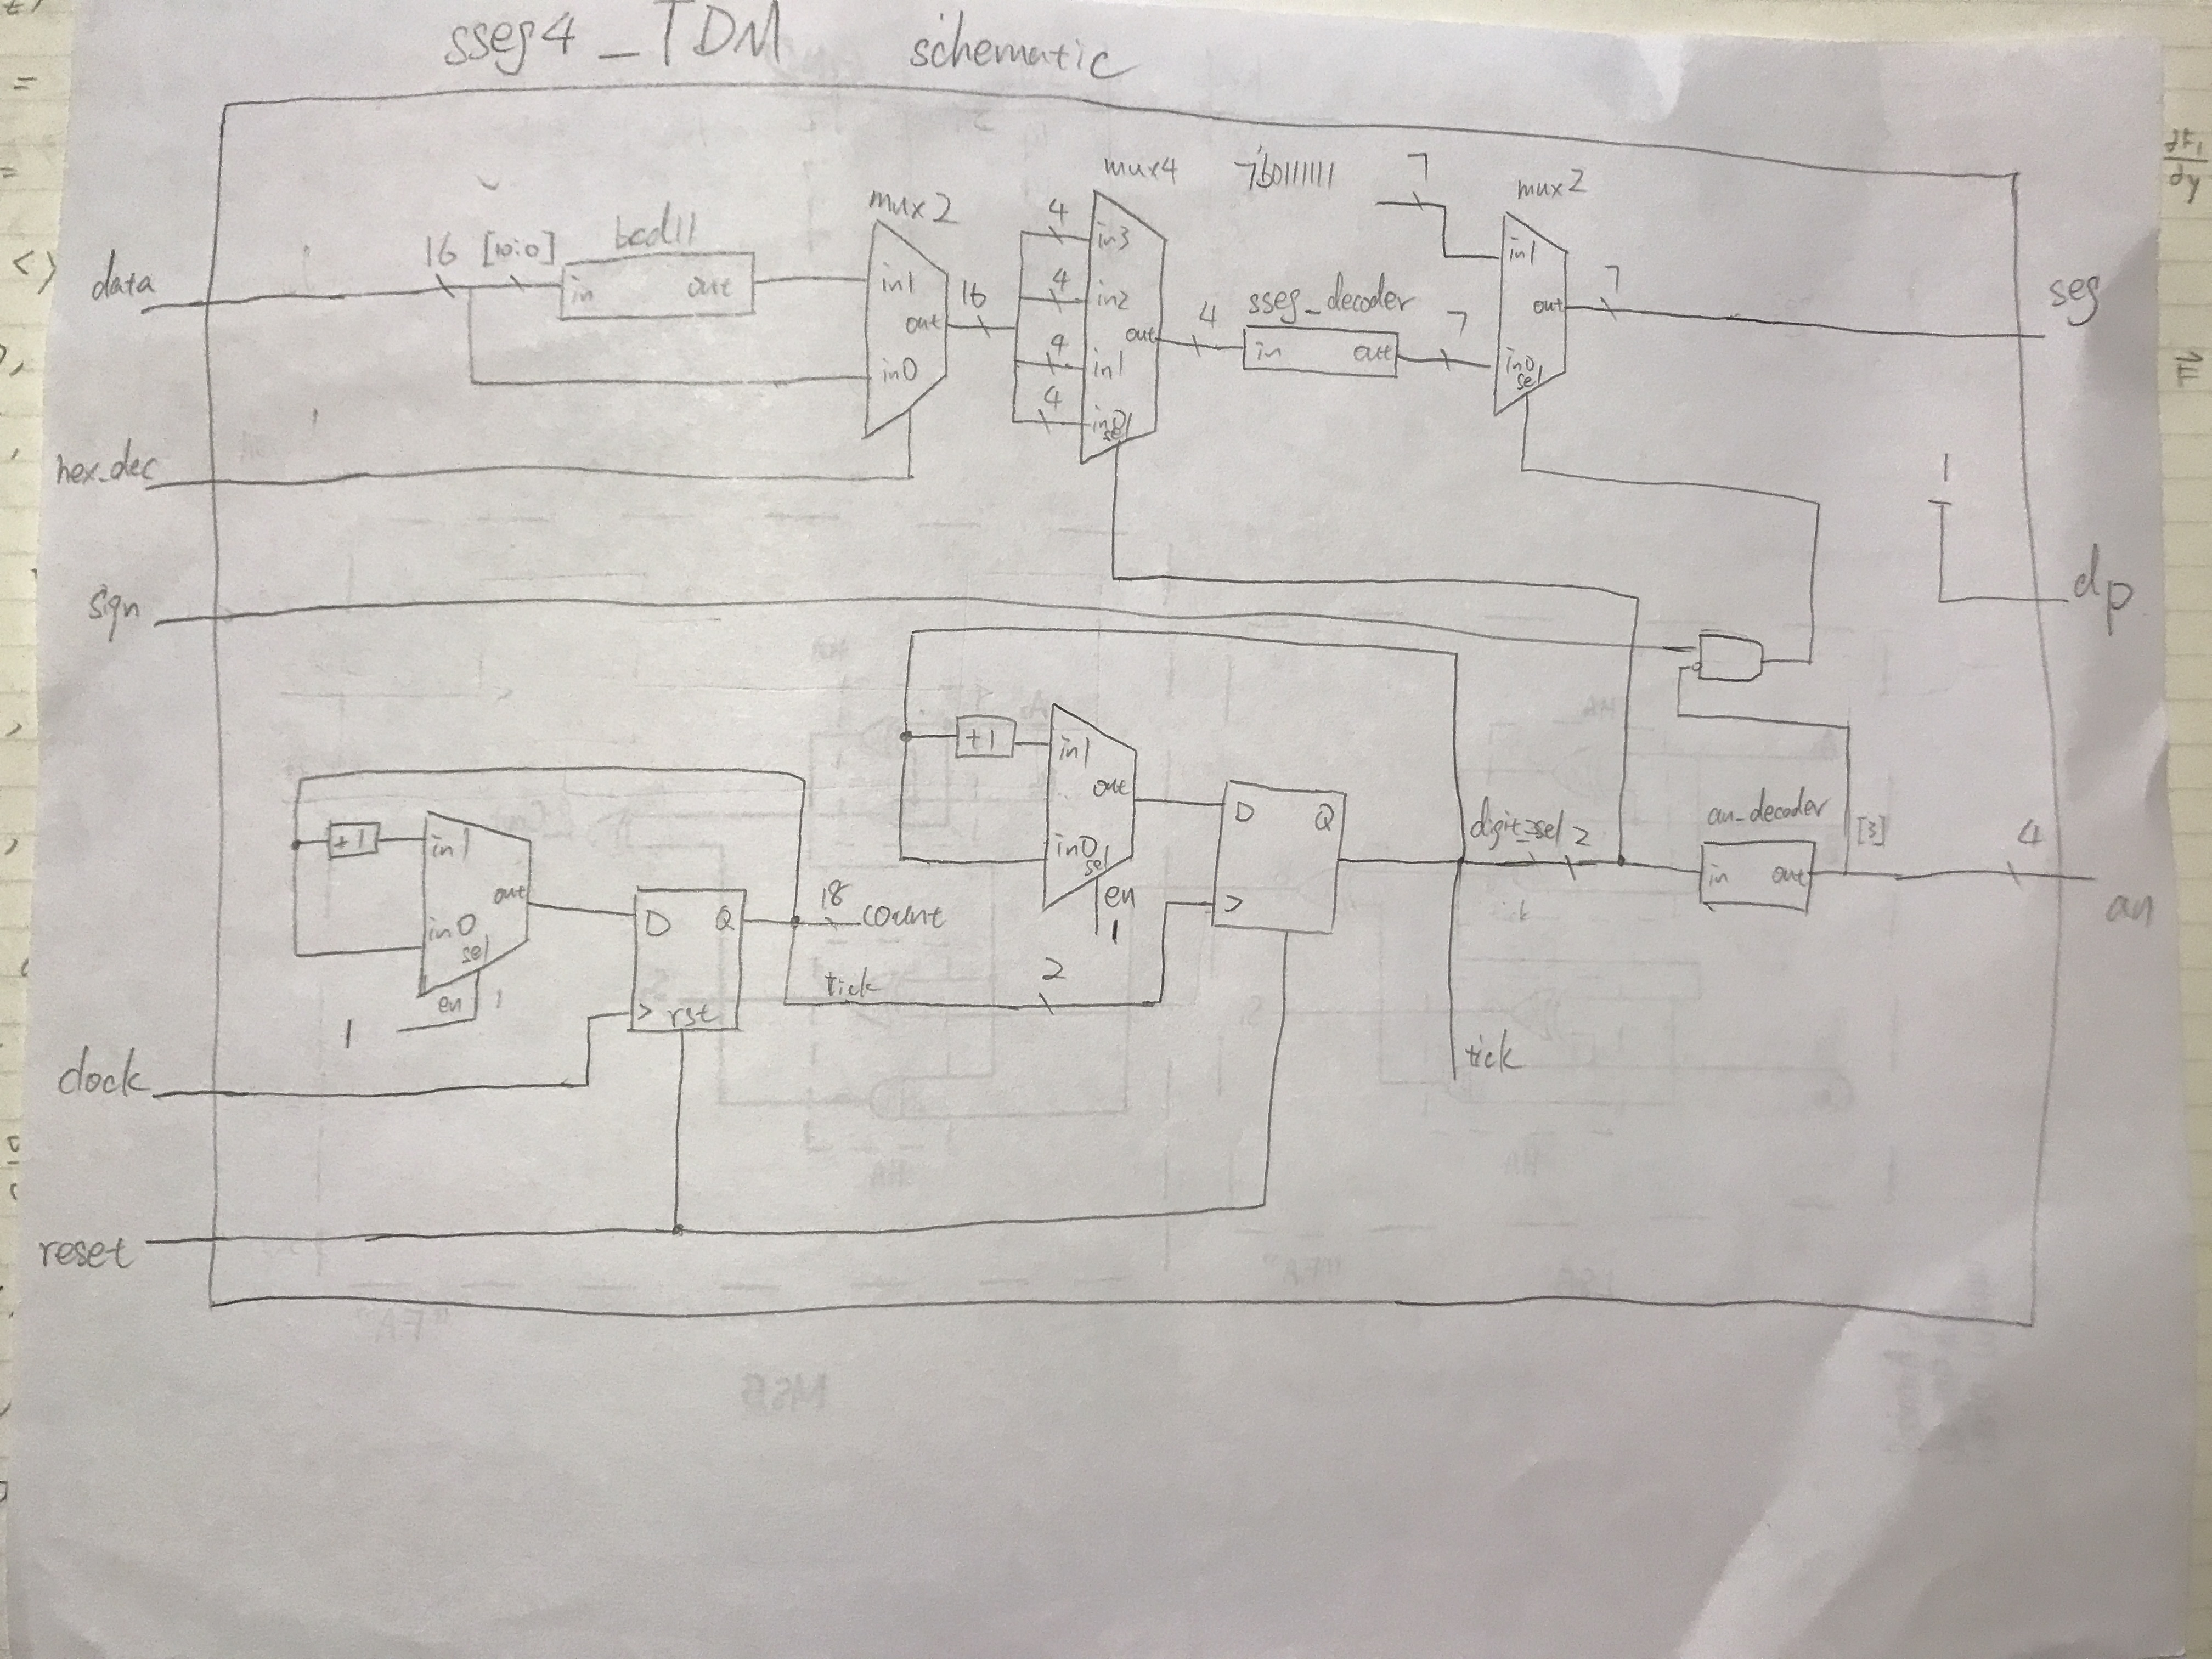
\includegraphics[width=\textwidth]{ssegTDM}
	\caption{Sseg4\_TDM schematic.}
	\label{fig:sseg4_TDM}			% label must be after caption
\end{figure}

\begin{figure}[ht]\centering
	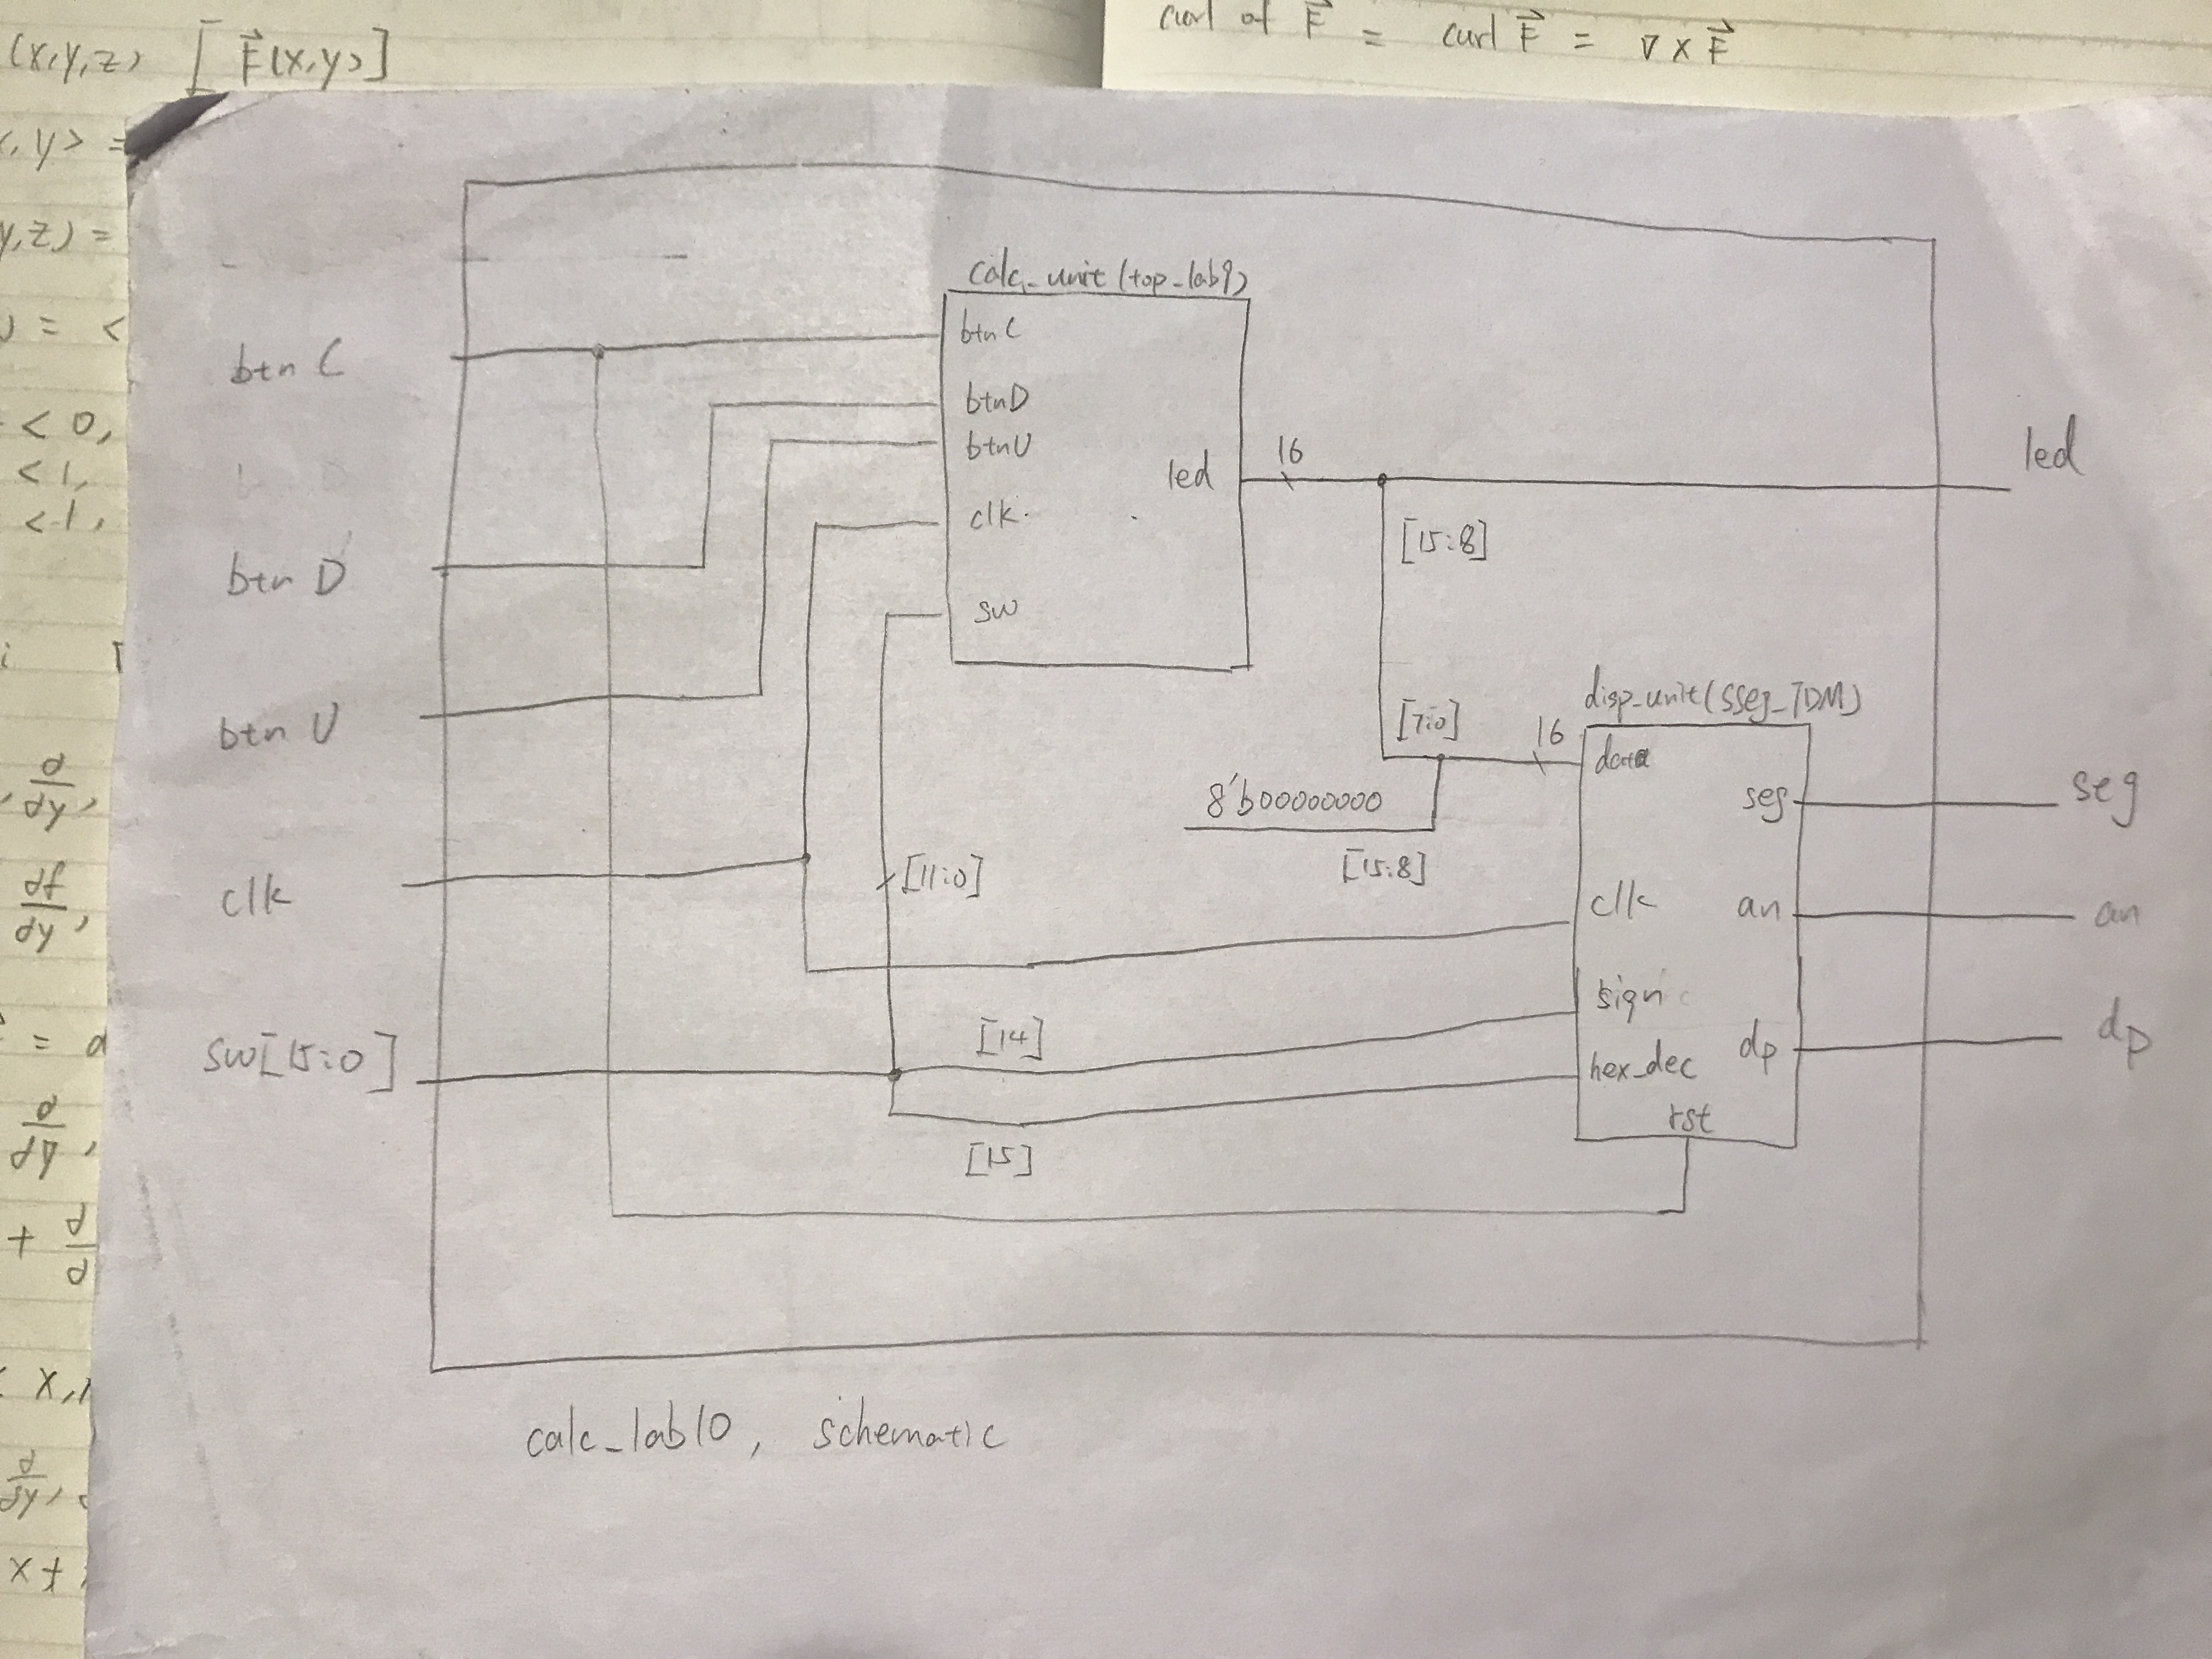
\includegraphics[width=\textwidth]{calclab10}
	\caption{Calc\_lab10 schematic.}
	\label{fig:calc_lab10}			% label must be after caption
\end{figure}
\clearpage

\section*{Q\&A}

\begin{enumerate}
	\item What are the three main “groups” of the RTL definition of sequential logic?
	
	The set of registers in the system.
	The operations that are performed on the data stored in the registers.
	The control that supervises the sequence of operations in the system.
	
	\item Copy Figure 10.3b onto your own paper (or do it electronically) and draw three boxes around the components that belong to each group. Include your annotated figure in your report.
	
\begin{figure}[ht]\centering
	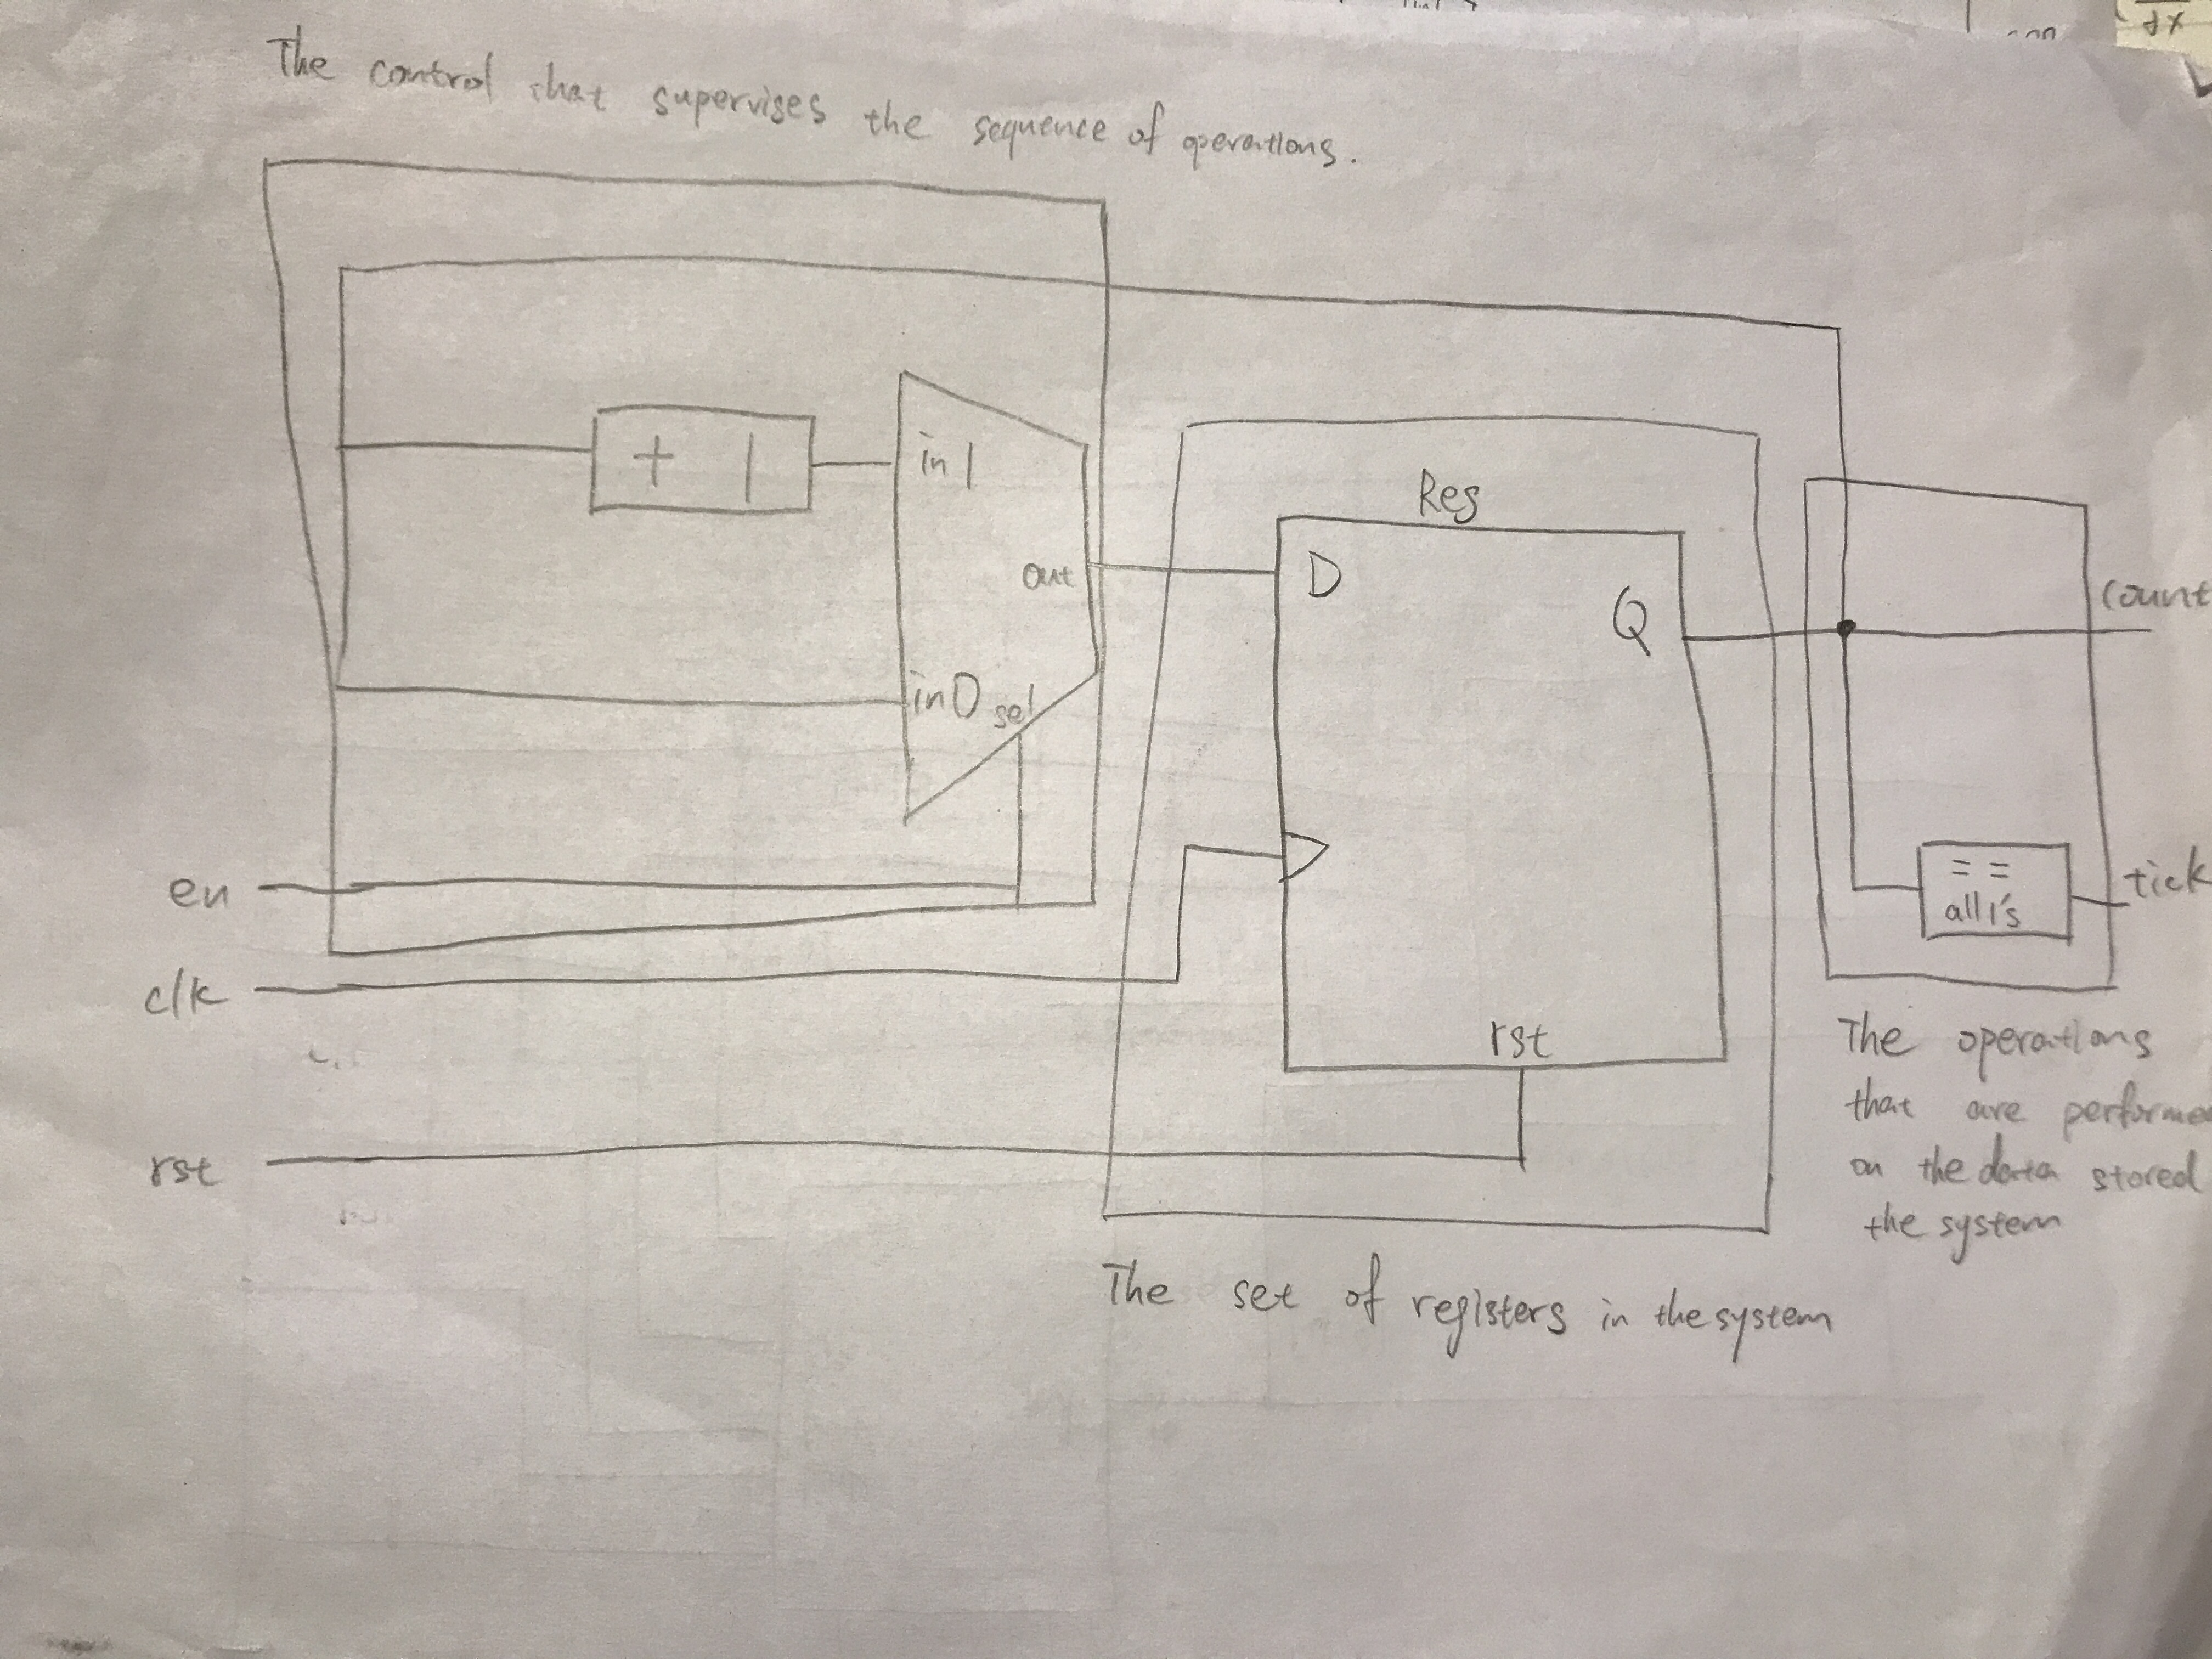
\includegraphics[width=\textwidth]{Q2}
	\caption{Three groups with the figure.}
	\label{fig:groups}			% label must be after caption
\end{figure}

	\item If instead of a counter, you wanted to make
	a shift register that moved the input bits
	from right to left (low to high). What would
	you put on the line Q next = /*???*/?
	
	Q\_next = Q\_reg - 1'b1;
	\clearpage
\end{enumerate}


\section*{Results}

\begin{figure}[ht]\centering
	\begin{tabular}{l|rrrrrrrrrrrrrrrr}
		Time (ns): & 0 &5& 10 &15& 20&25 & 30&35&40&45&50&55&60&65&70&75 \\
		\midrule
		clk & 0 & 1 & 0 & 1 &0 &1 & 0& 1& 0 &1 & 0 & 1& 0 & 1& 0 & 1\\
		en & 0 & 1 & 1 & 1  & 1& 1 & 0 & 0 & 1 & 1 &0 & 0& 1 & 1 & 0 & 0\\
		rst & 0& 1& 0 & 0 & 0 & 0 &0 & 0 & 0 & 0 & 0 & 0 & 0 & 0 & 0 & 0\\
		\midrule
		count & X & 0 & 0 & 1 & 1 & 2 & 2 & 2 & 2 & 3 & 3 & 3 & 3 & 4 & 4 & 4\\
		s & X & 0 & 0 & 0 & 0 & 0 & 0 & 0 & 0 & 0 & 0 & 0 & 0 & 0 & 0 &0 \\
		\bottomrule
	\end{tabular}\medskip
	
	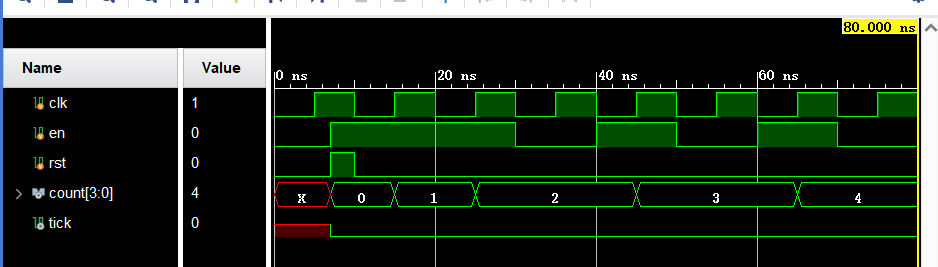
\includegraphics{countertest}
	\caption{counter simulation waveform and ERT}
	\label{fig:counter wave and ERT}
\end{figure}

\begin{figure}[ht]\centering
	\begin{tabular}{l|rrrrrrr}
		Time (ns): & 0-20 &20 - 60& 60 - 140 & 140 -300& 300-460 & 460 -780 & 780 -1000\\
		\midrule
		data & 2 & 1 & 2 & 2 & 3 &3& 4\\
		hex\_dec & 0 & 1 & 0 & 1  & 0 & 1 & 0 \\
		sign & 0& 0& 0 & 0 & 0 & 0 & 0\\
		\midrule
		count & 23 & 79 & 24&24 & 30 & 30 & 19 \\
		an & X & X & X & X & e & e & e \\
		dp & 1 & 1 & 1 & 1 & 1 & 1 & 1\\
		\bottomrule
	\end{tabular}\medskip
	
	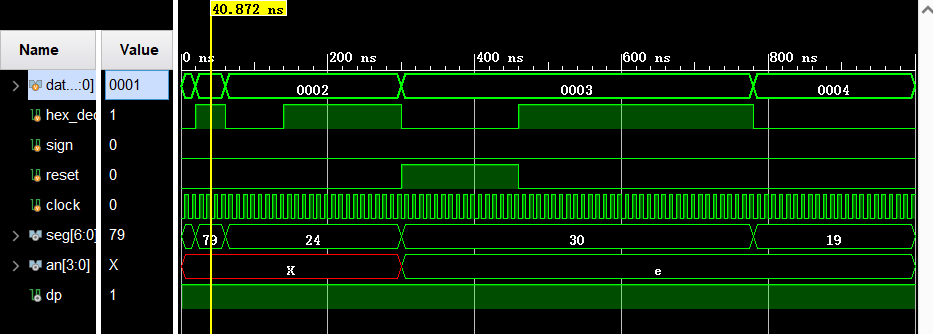
\includegraphics{ssegtest}
	\caption{sseg4\_TDM simulation waveform and ERT}
	\label{fig:sseg4_TDM wave and ERT}
\end{figure}

\begin{figure}[ht]\centering
	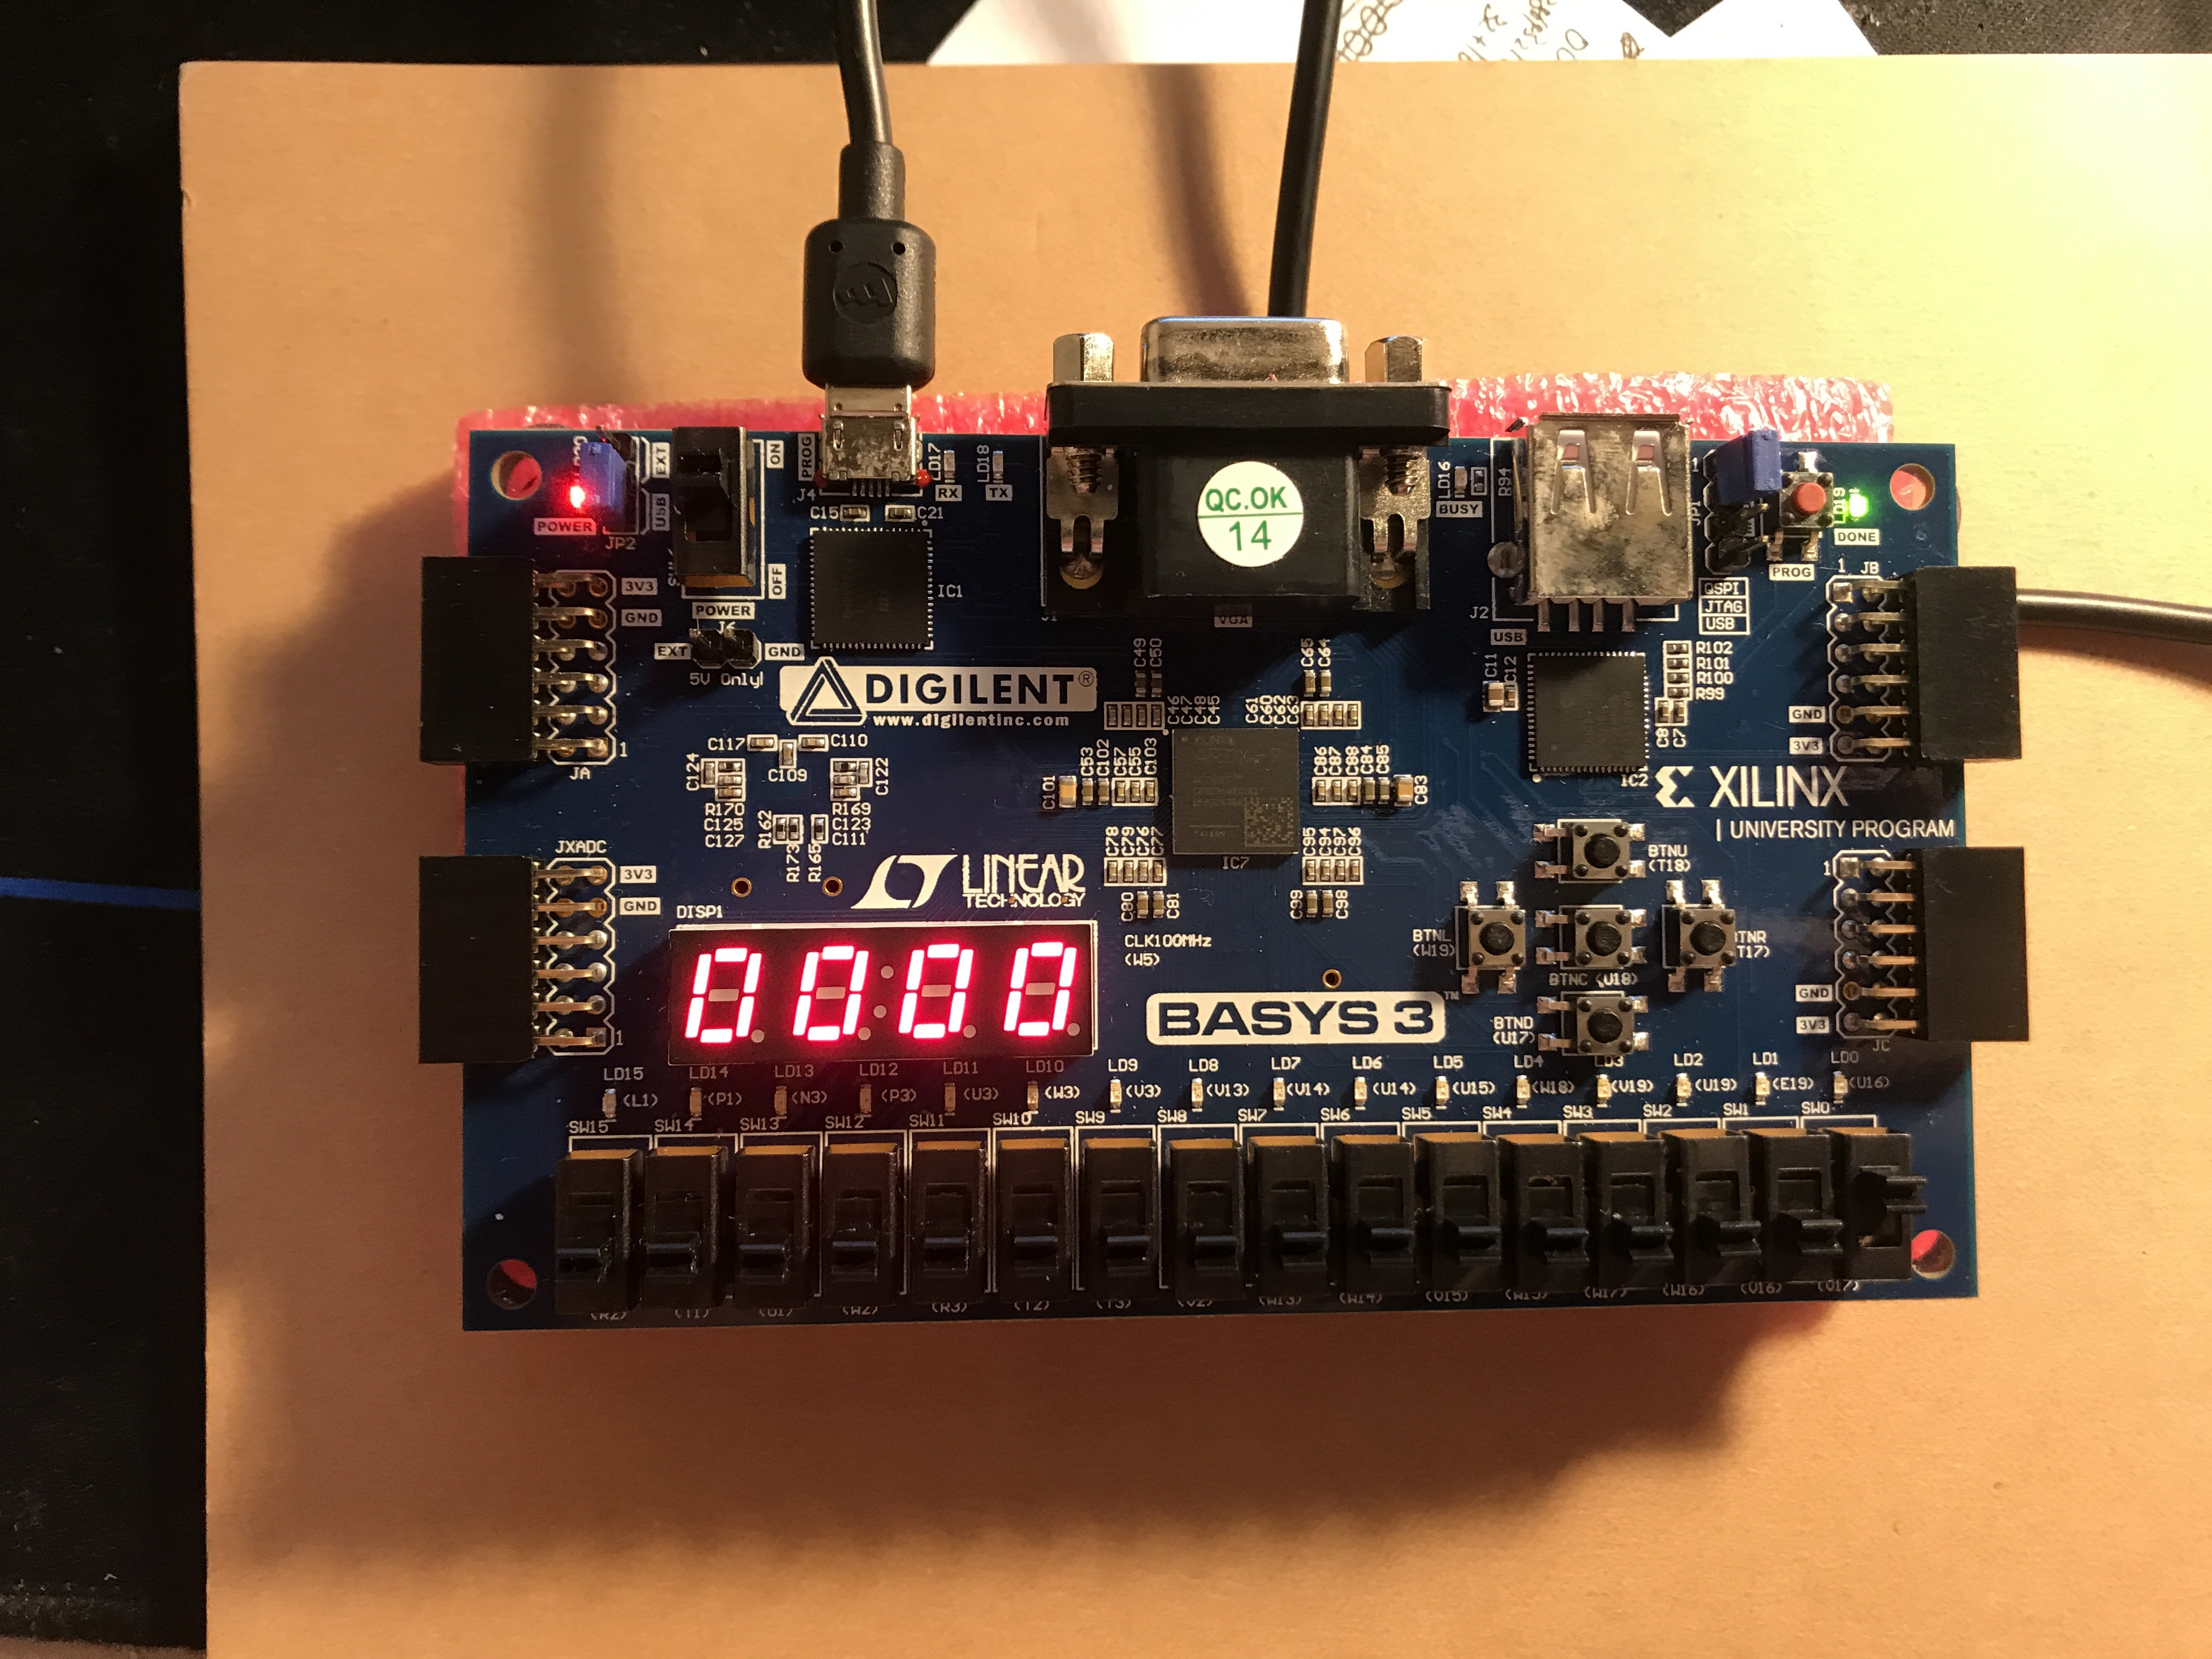
\includegraphics[width=0.5\textwidth]{board1}
	\caption{Board display 1.}
	\label{fig:board 1}			% label must be after caption
\end{figure}

\begin{figure}[ht]\centering
	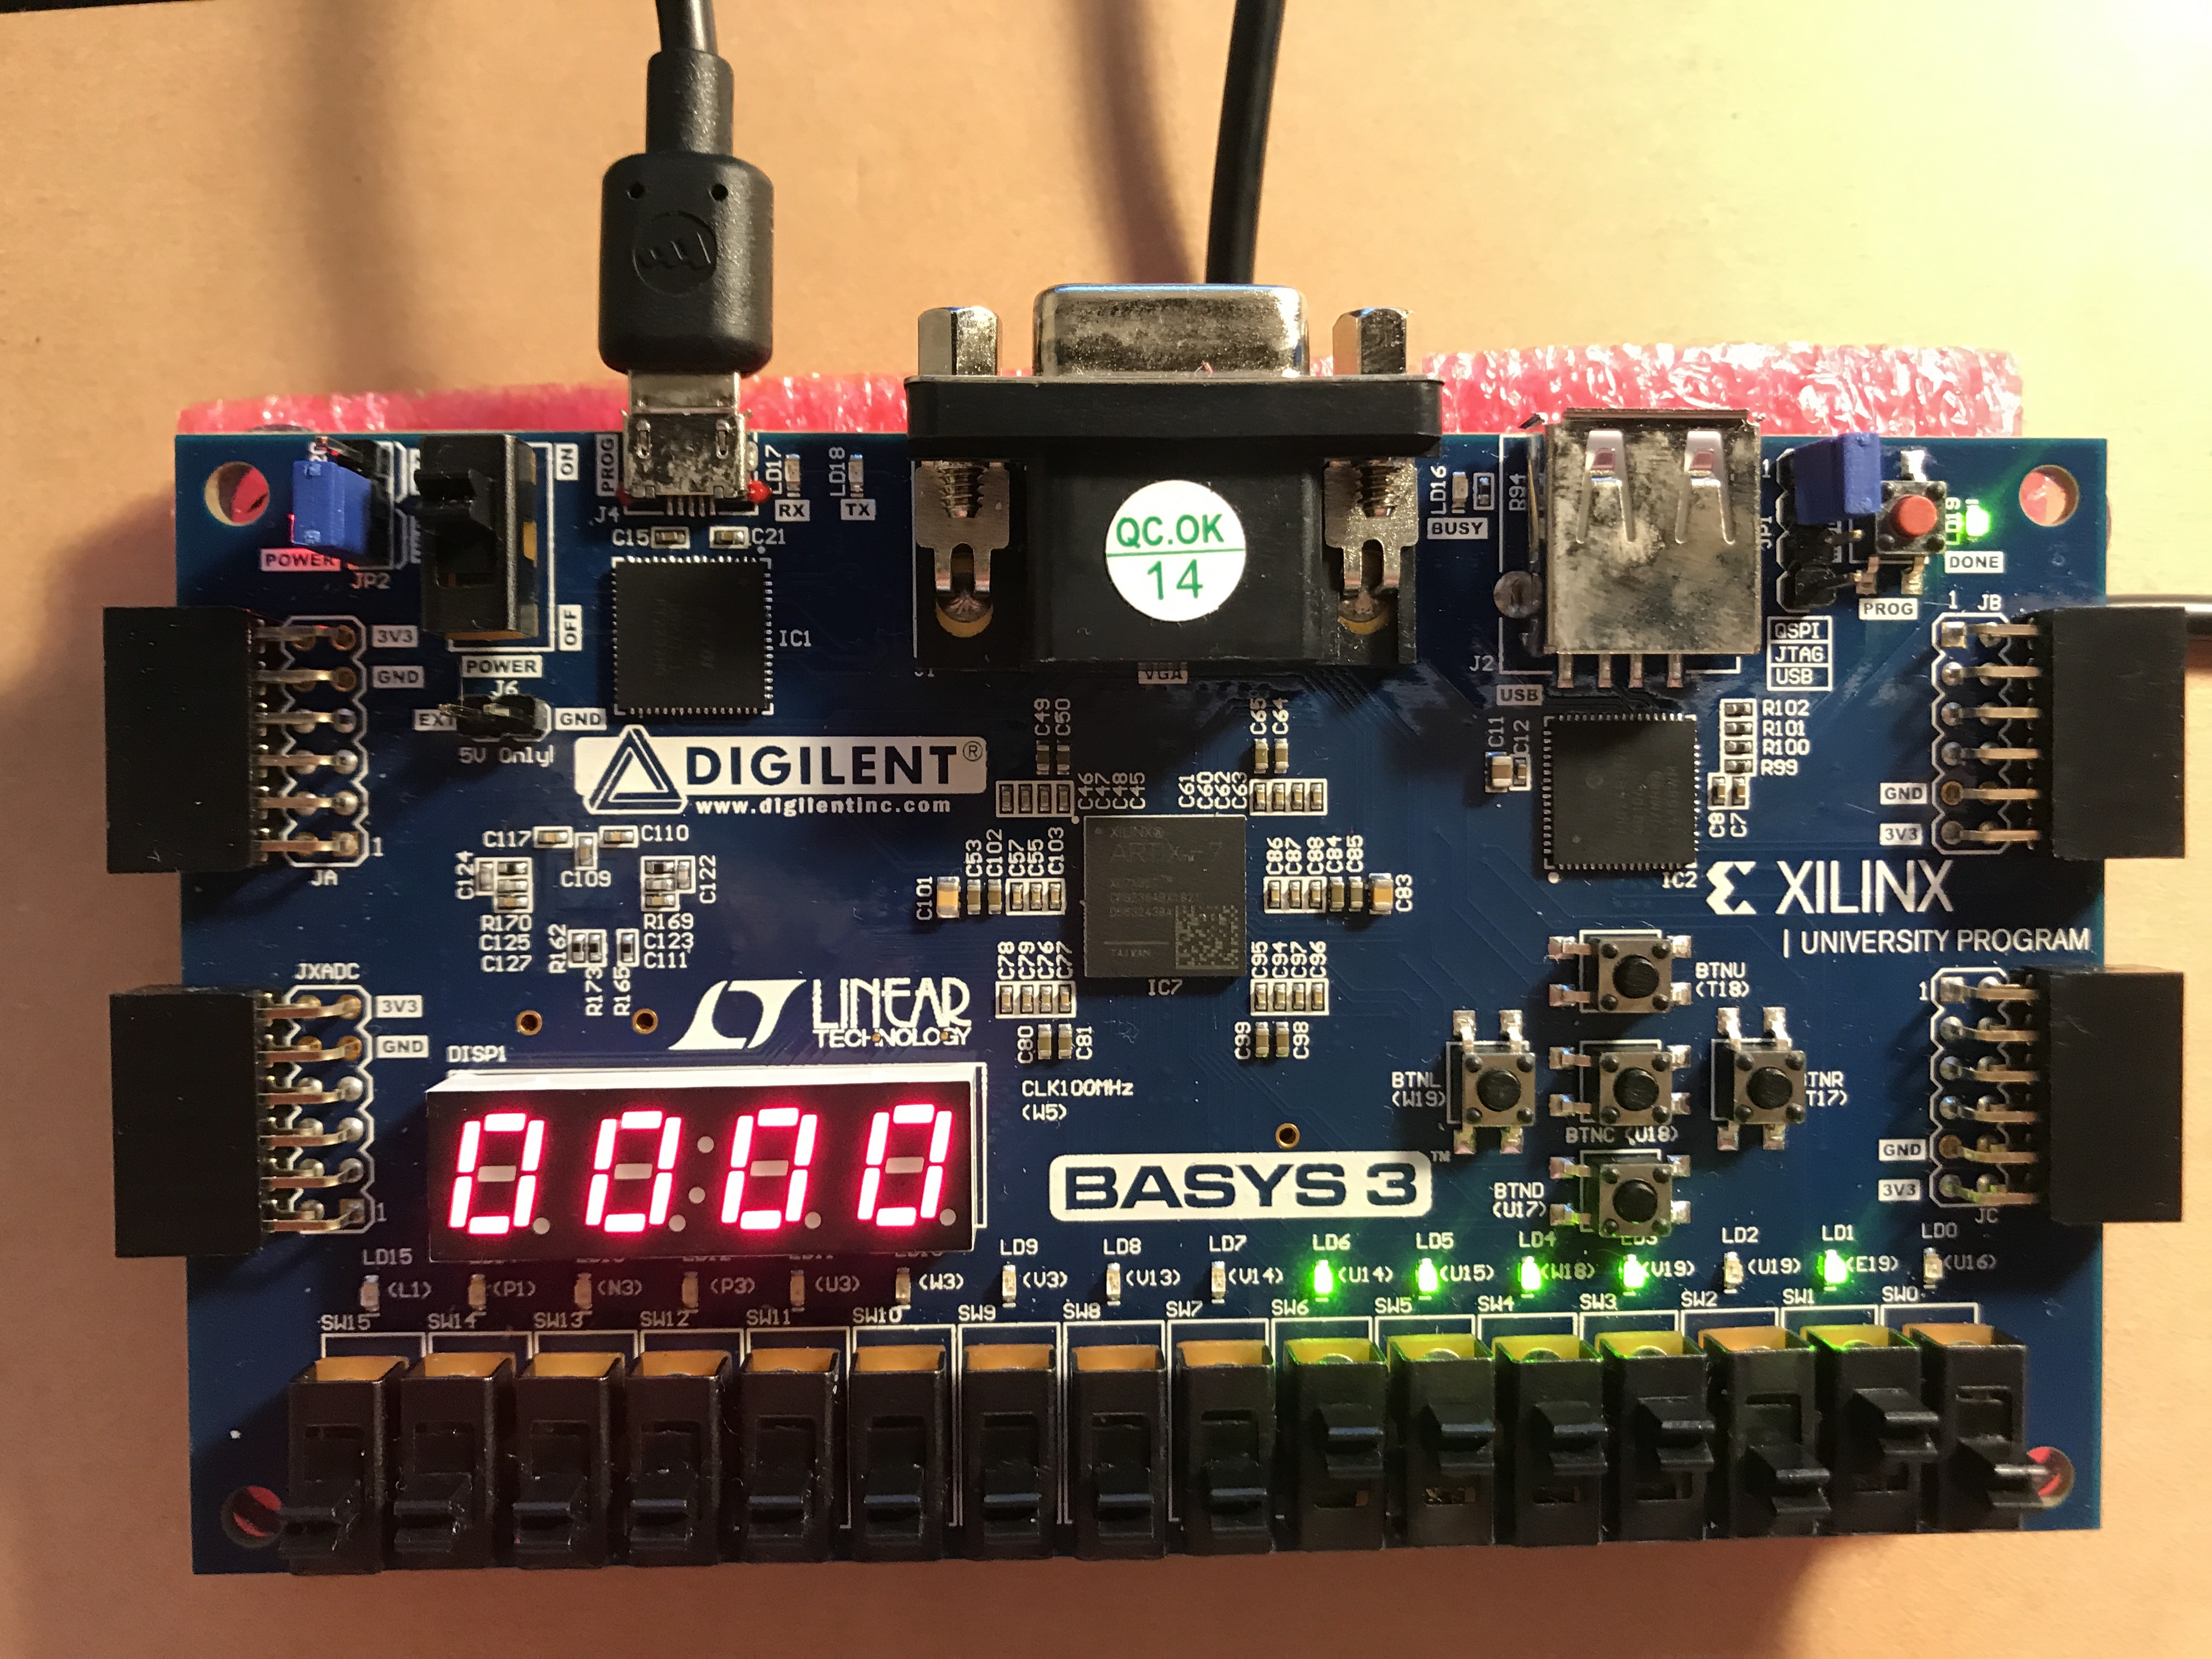
\includegraphics[width=0.5\textwidth]{board2}
	\caption{Board display.}
	\label{fig:board 2}			% label must be after caption
\end{figure}

\begin{figure}[ht]\centering
	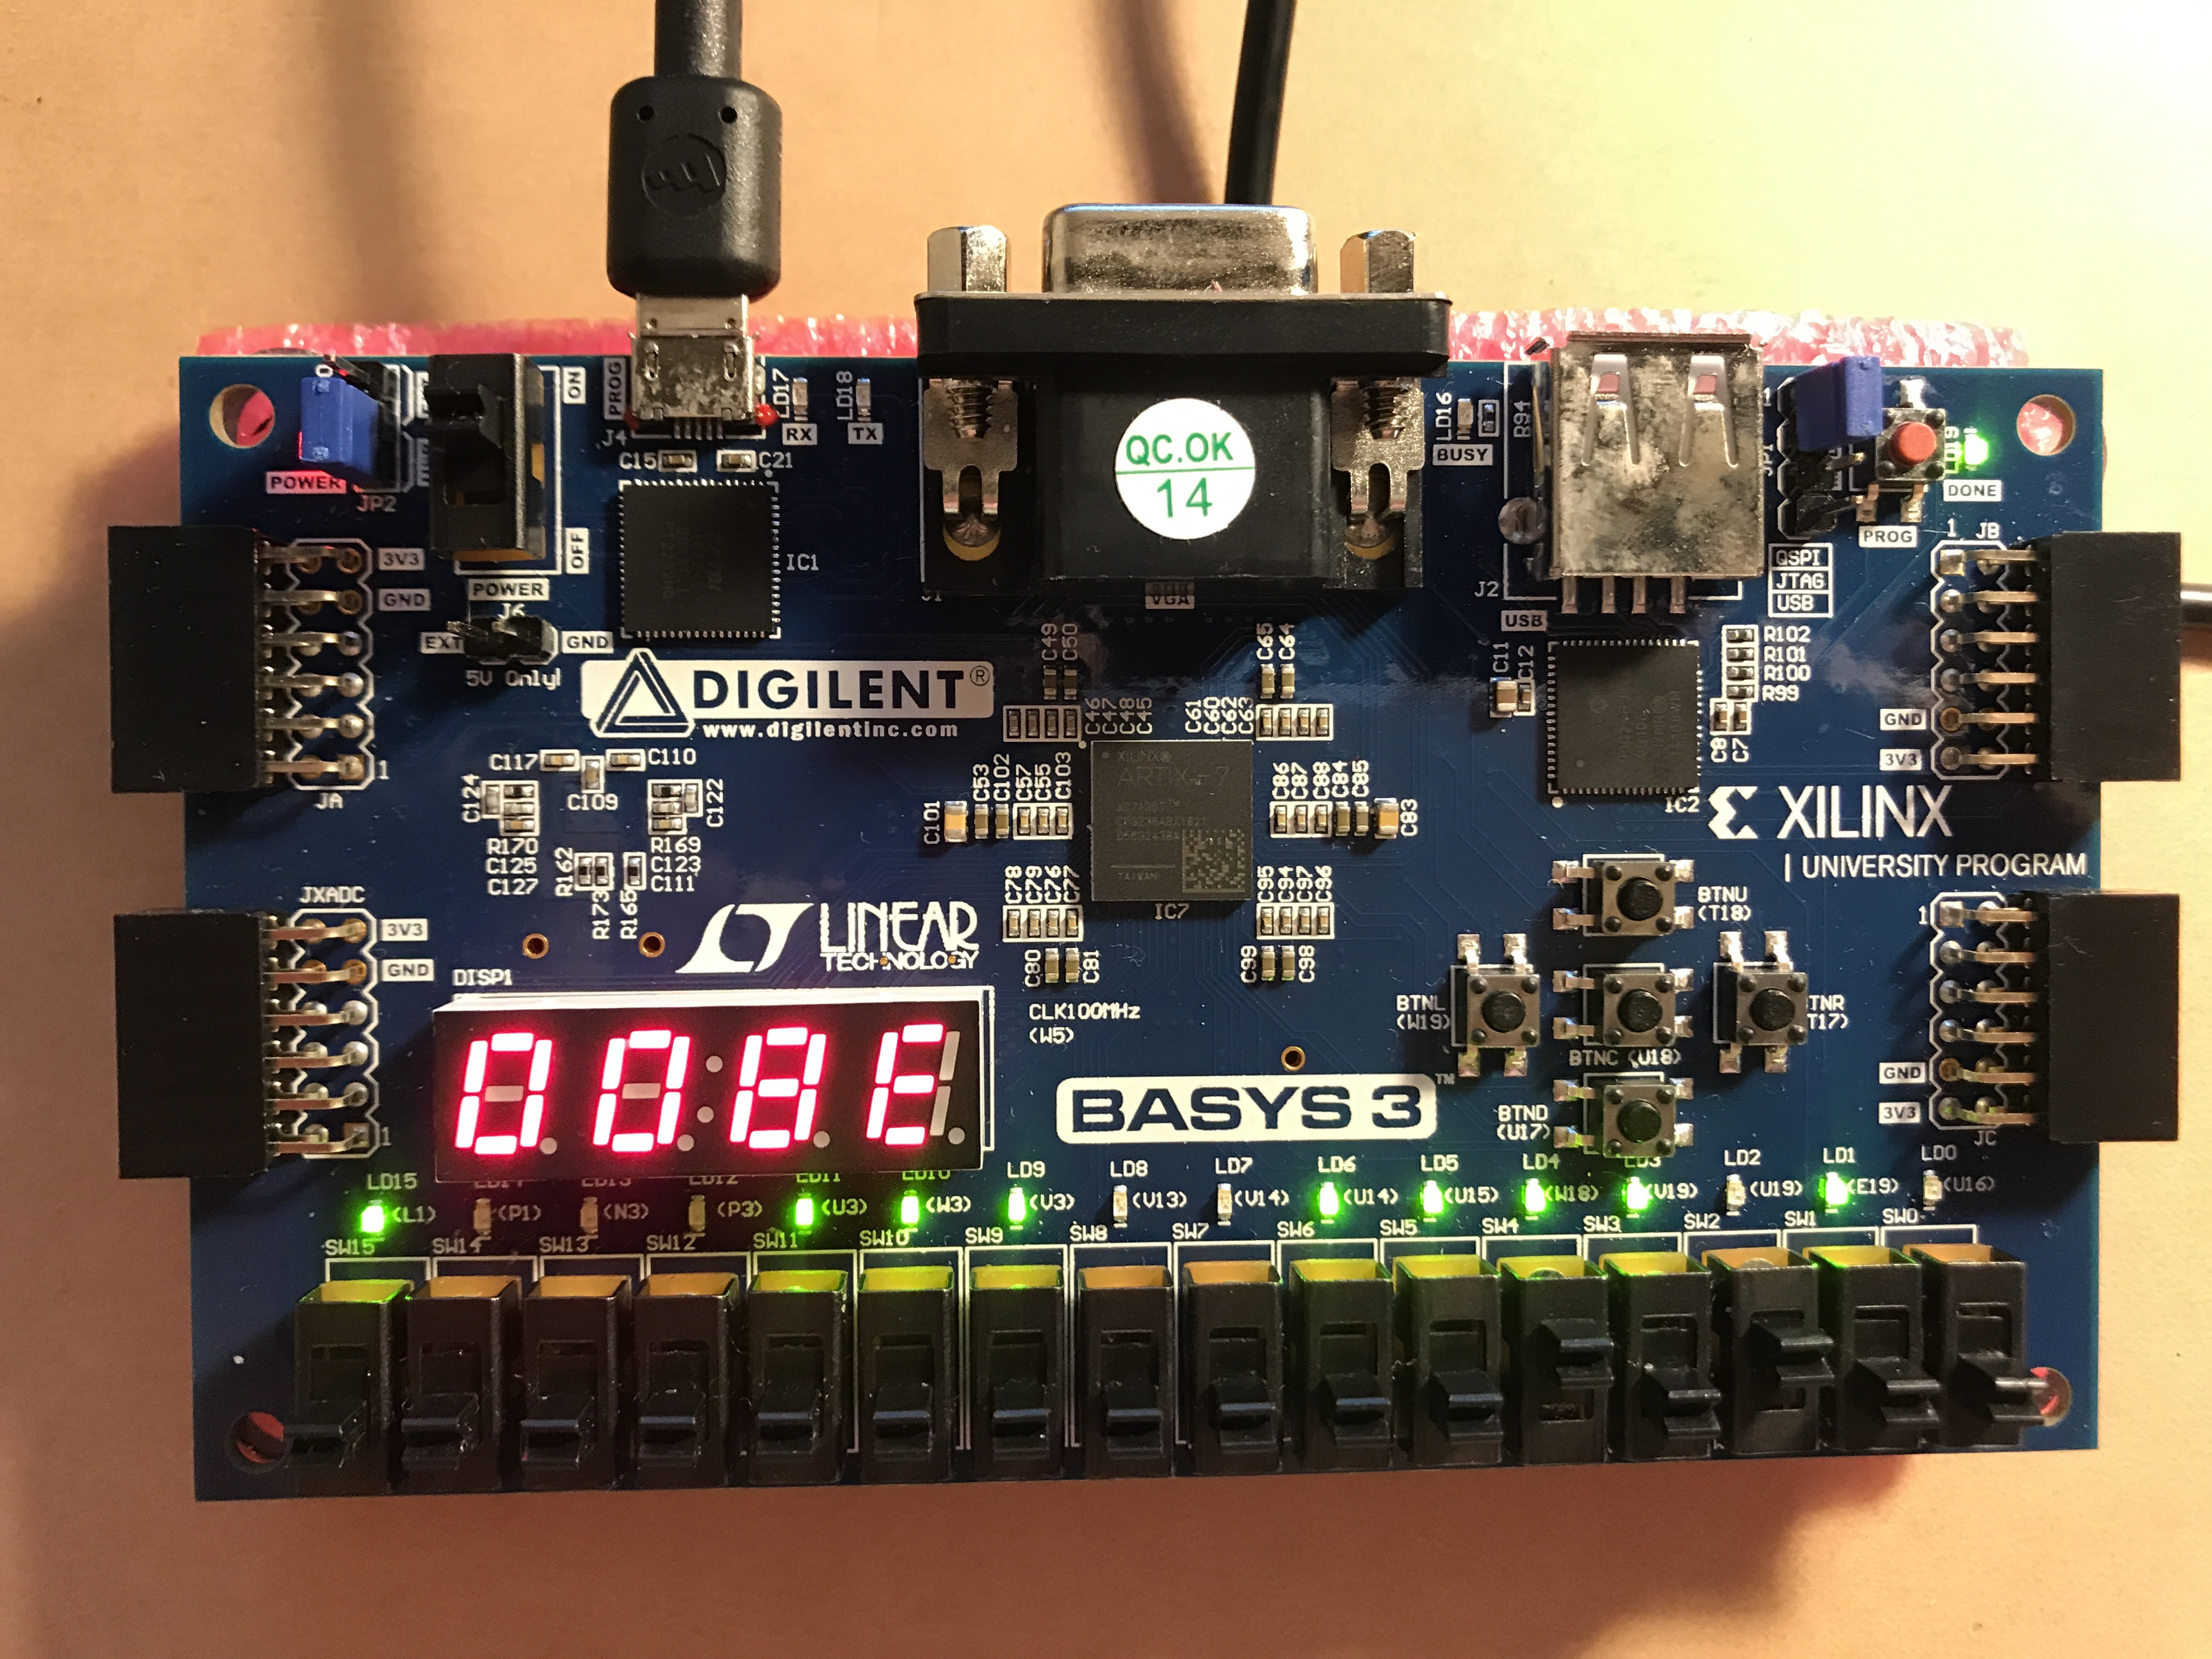
\includegraphics[width=0.5\textwidth]{board3}
	\caption{Board display 3.}
	\label{fig:board 3}			% label must be after caption
\end{figure}

\begin{figure}[ht]\centering
	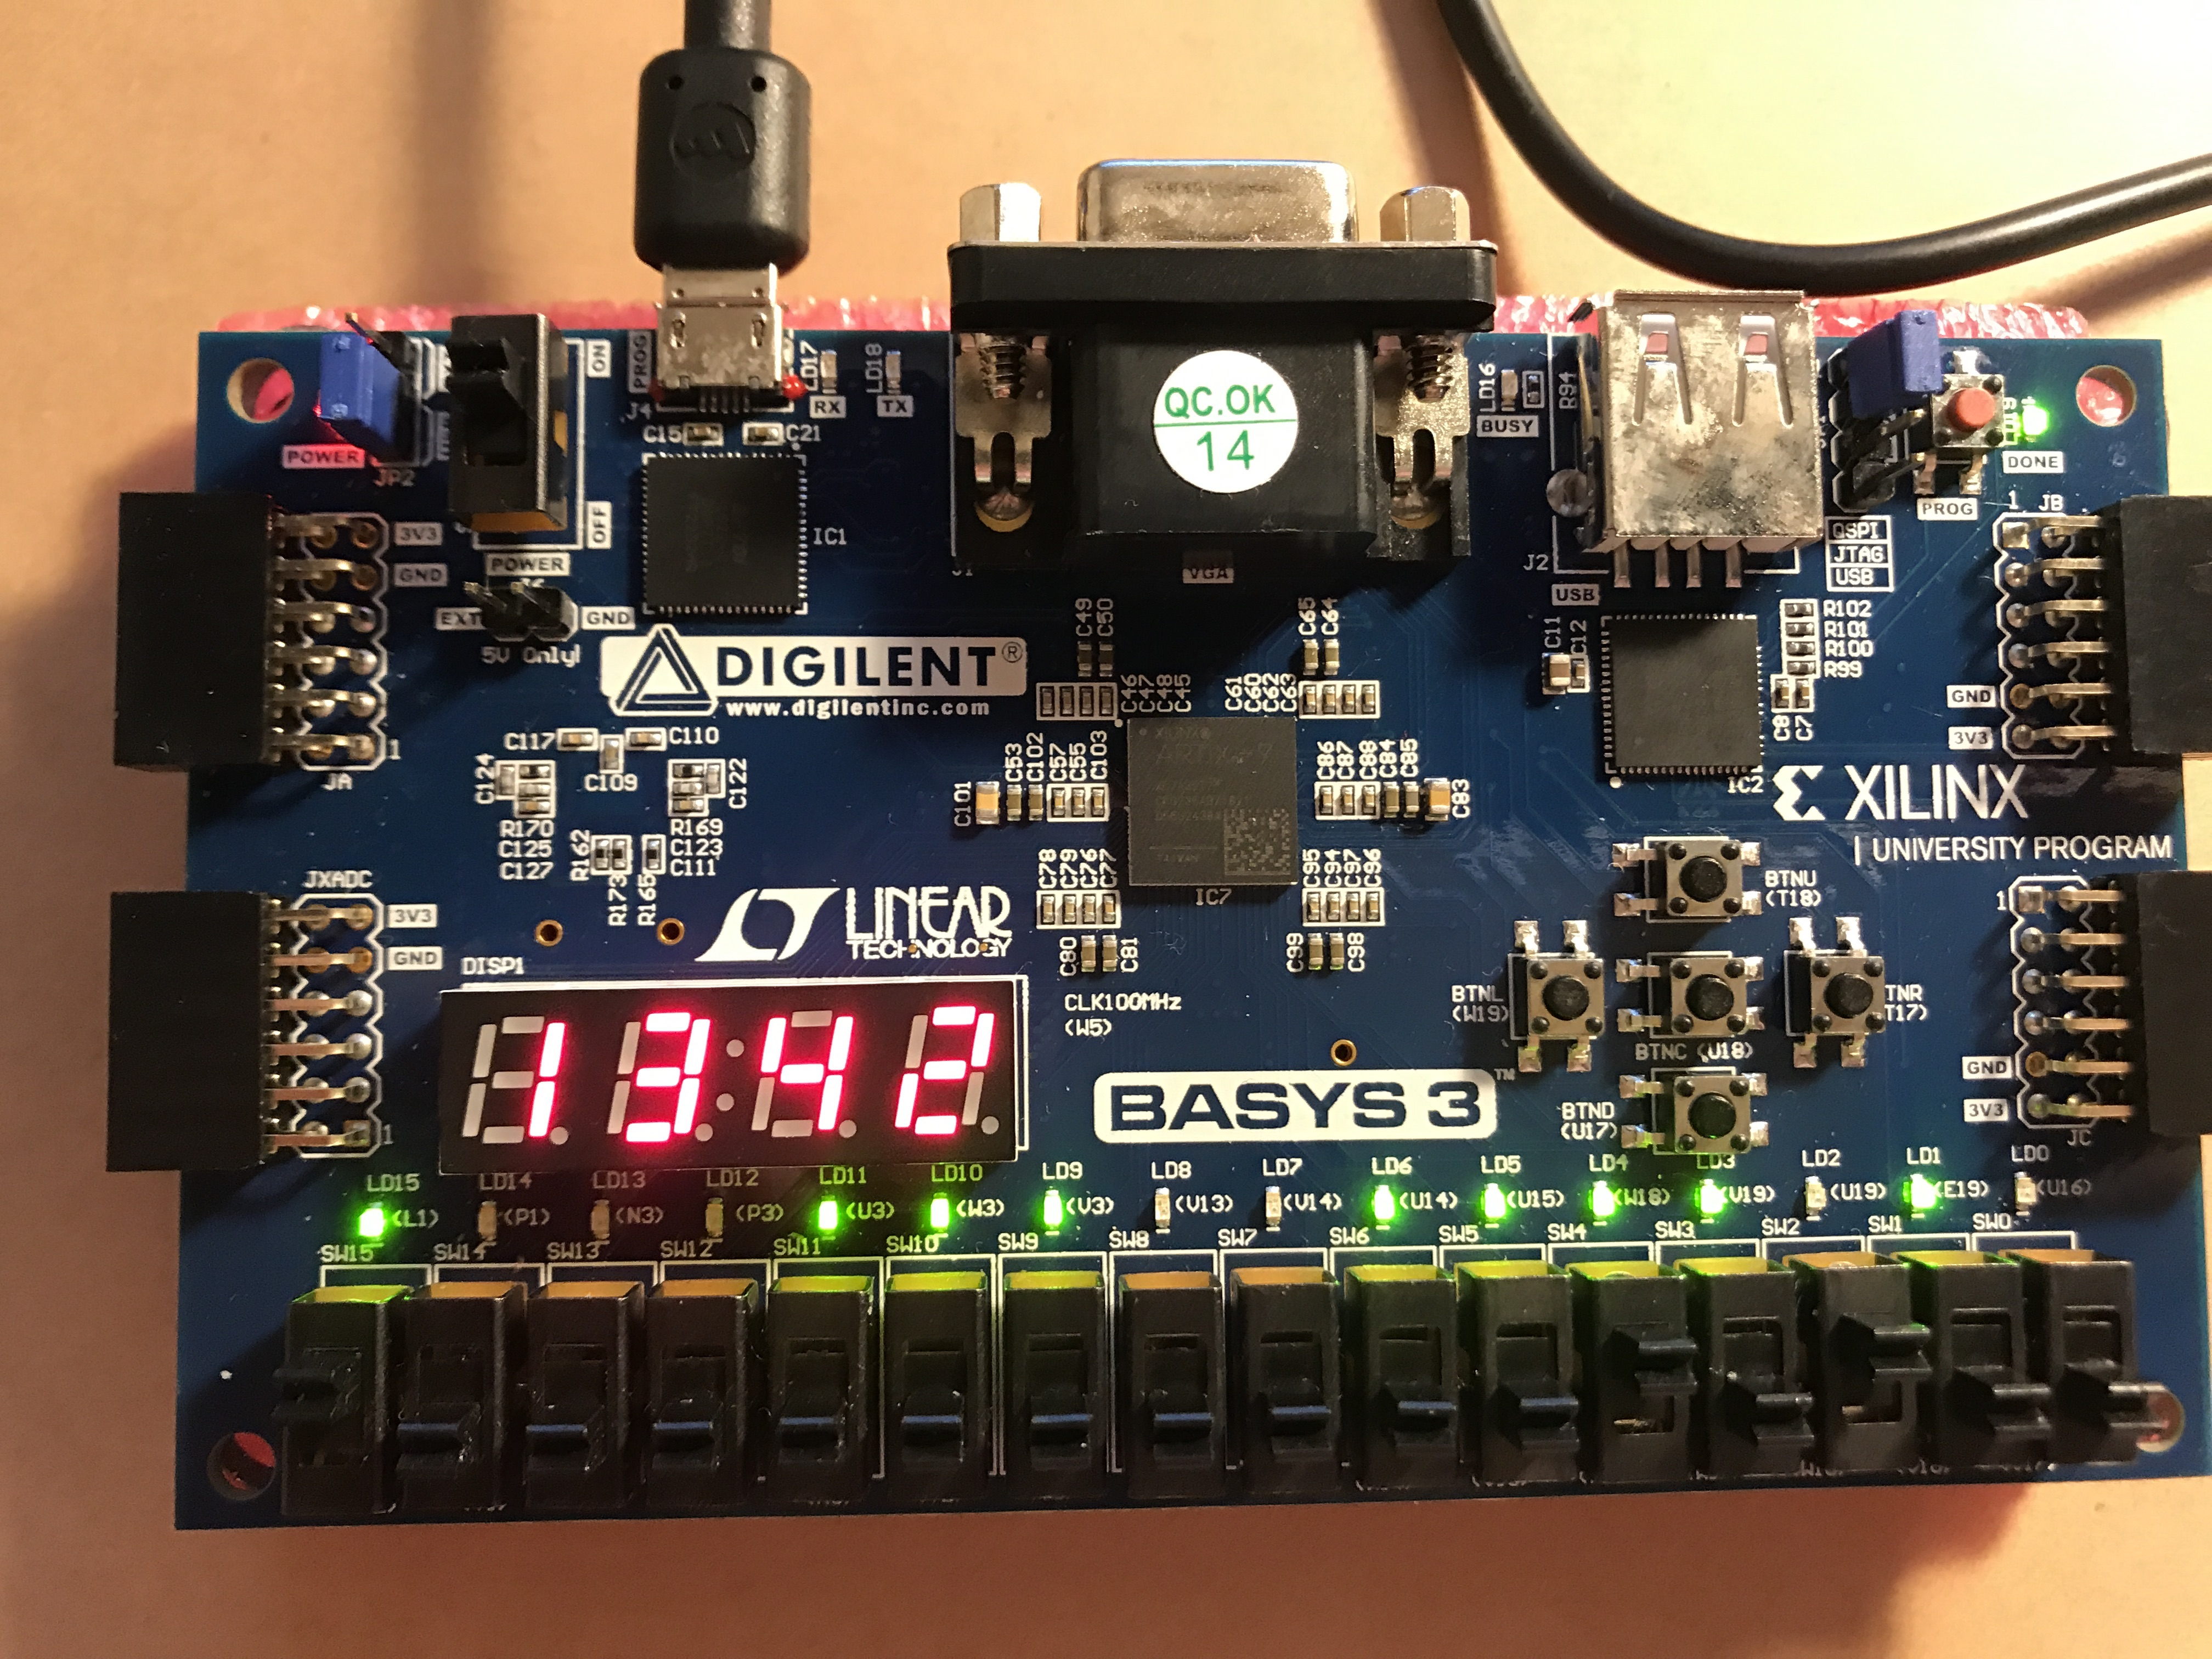
\includegraphics[width=0.5\textwidth]{board4}
	\caption{Board display 4.}
	\label{fig:board 4}			% label must be after caption
\end{figure}

\begin{figure}[ht]\centering
	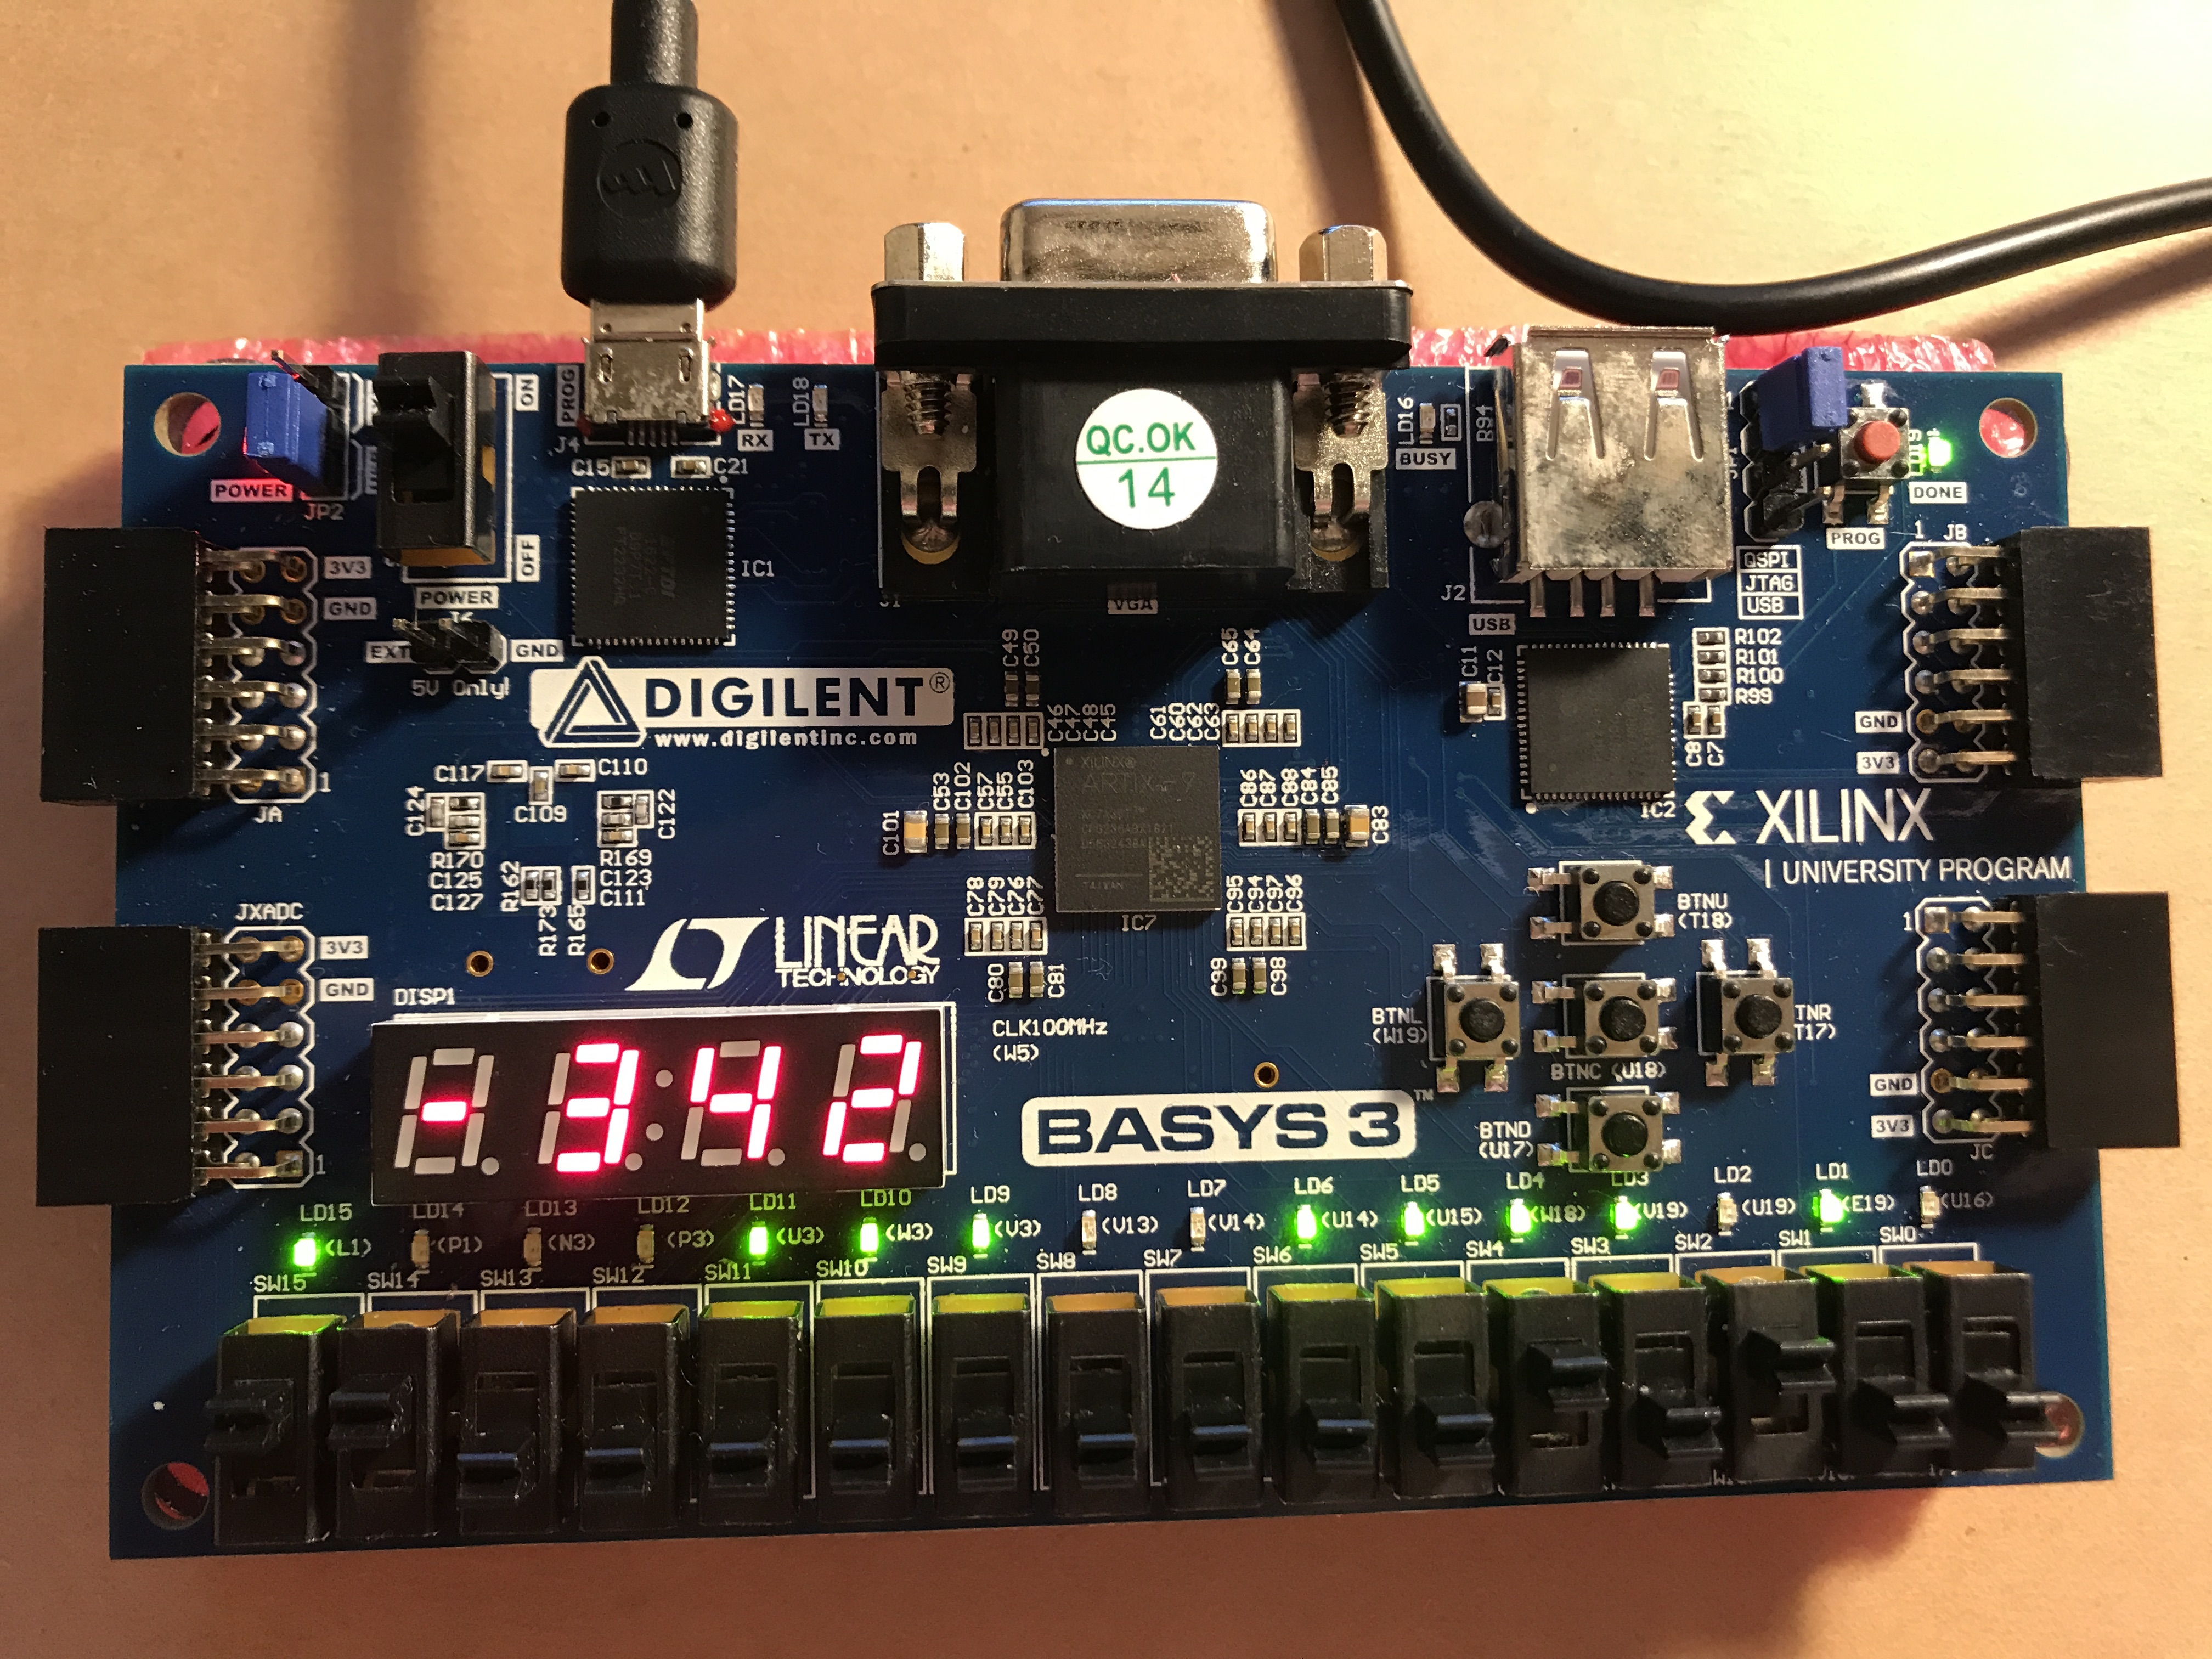
\includegraphics[width=0.5\textwidth]{board5}
	\caption{Board display 5.}
	\label{fig:board 5}			% label must be after caption
\end{figure}

\begin{figure}[ht]\centering
	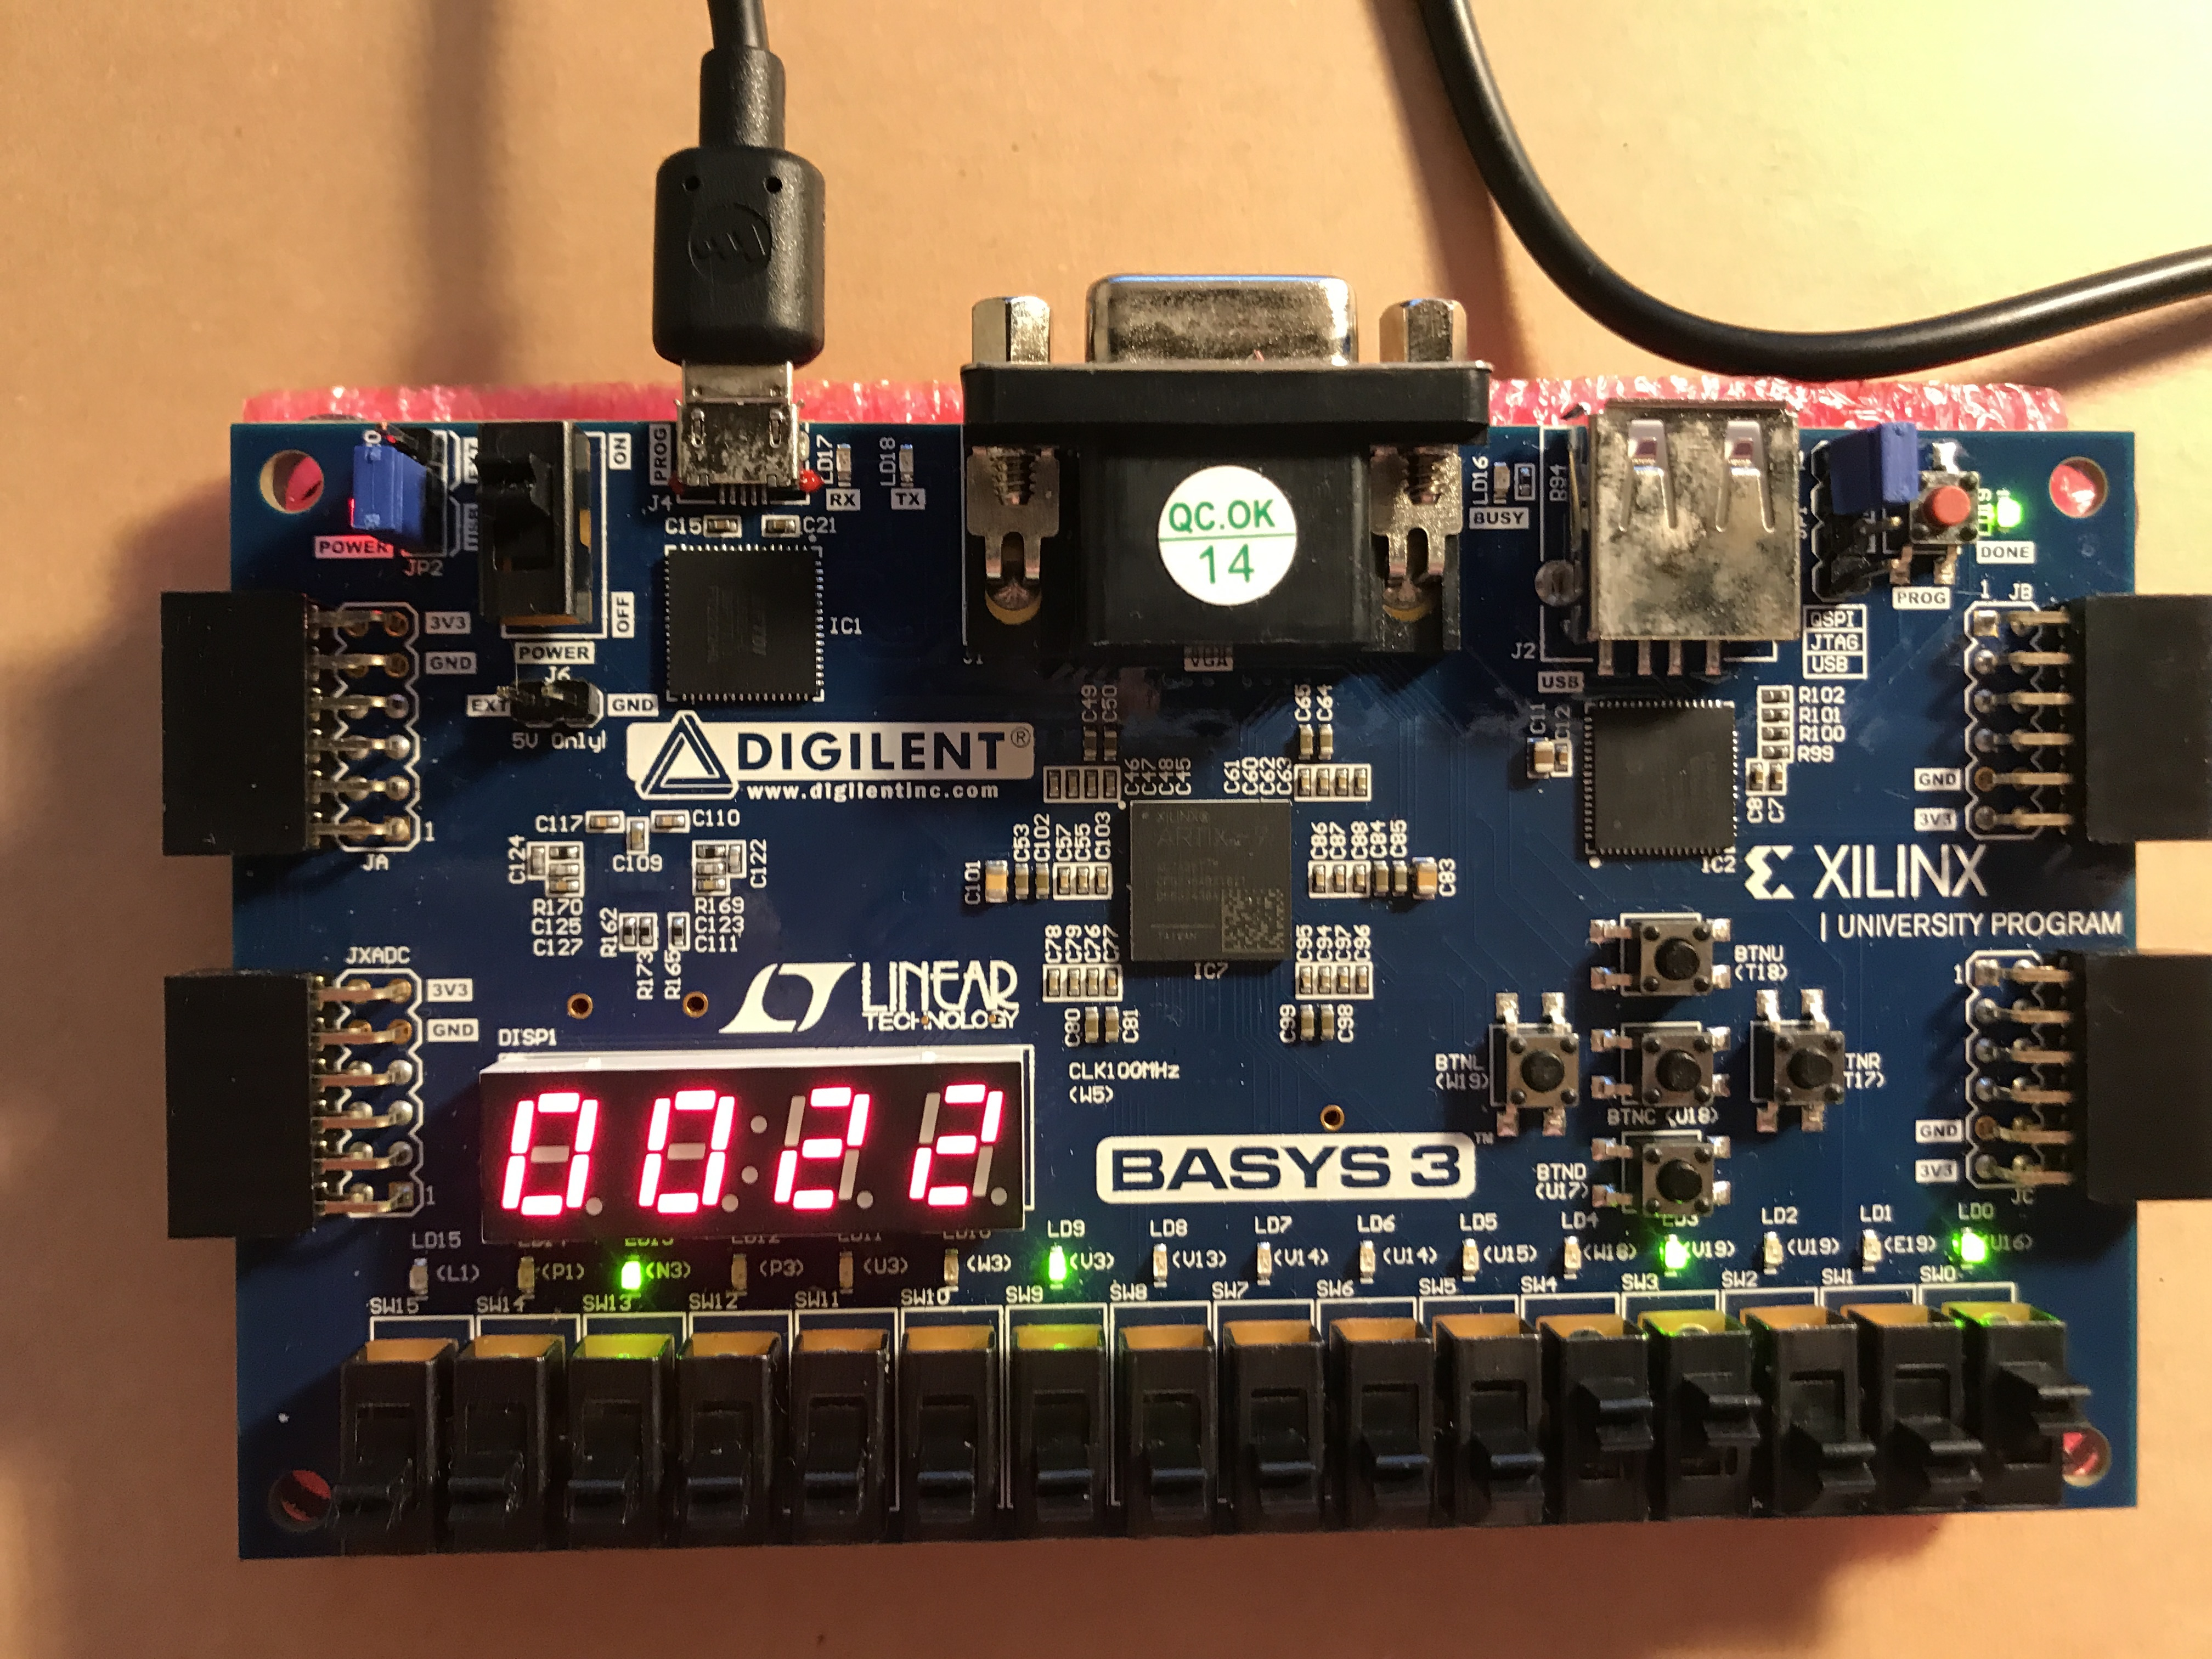
\includegraphics[width=0.5\textwidth]{board6}
	\caption{Board display 6.}
	\label{fig:board 6}			% label must be after caption
\end{figure}

\begin{figure}[ht]\centering
	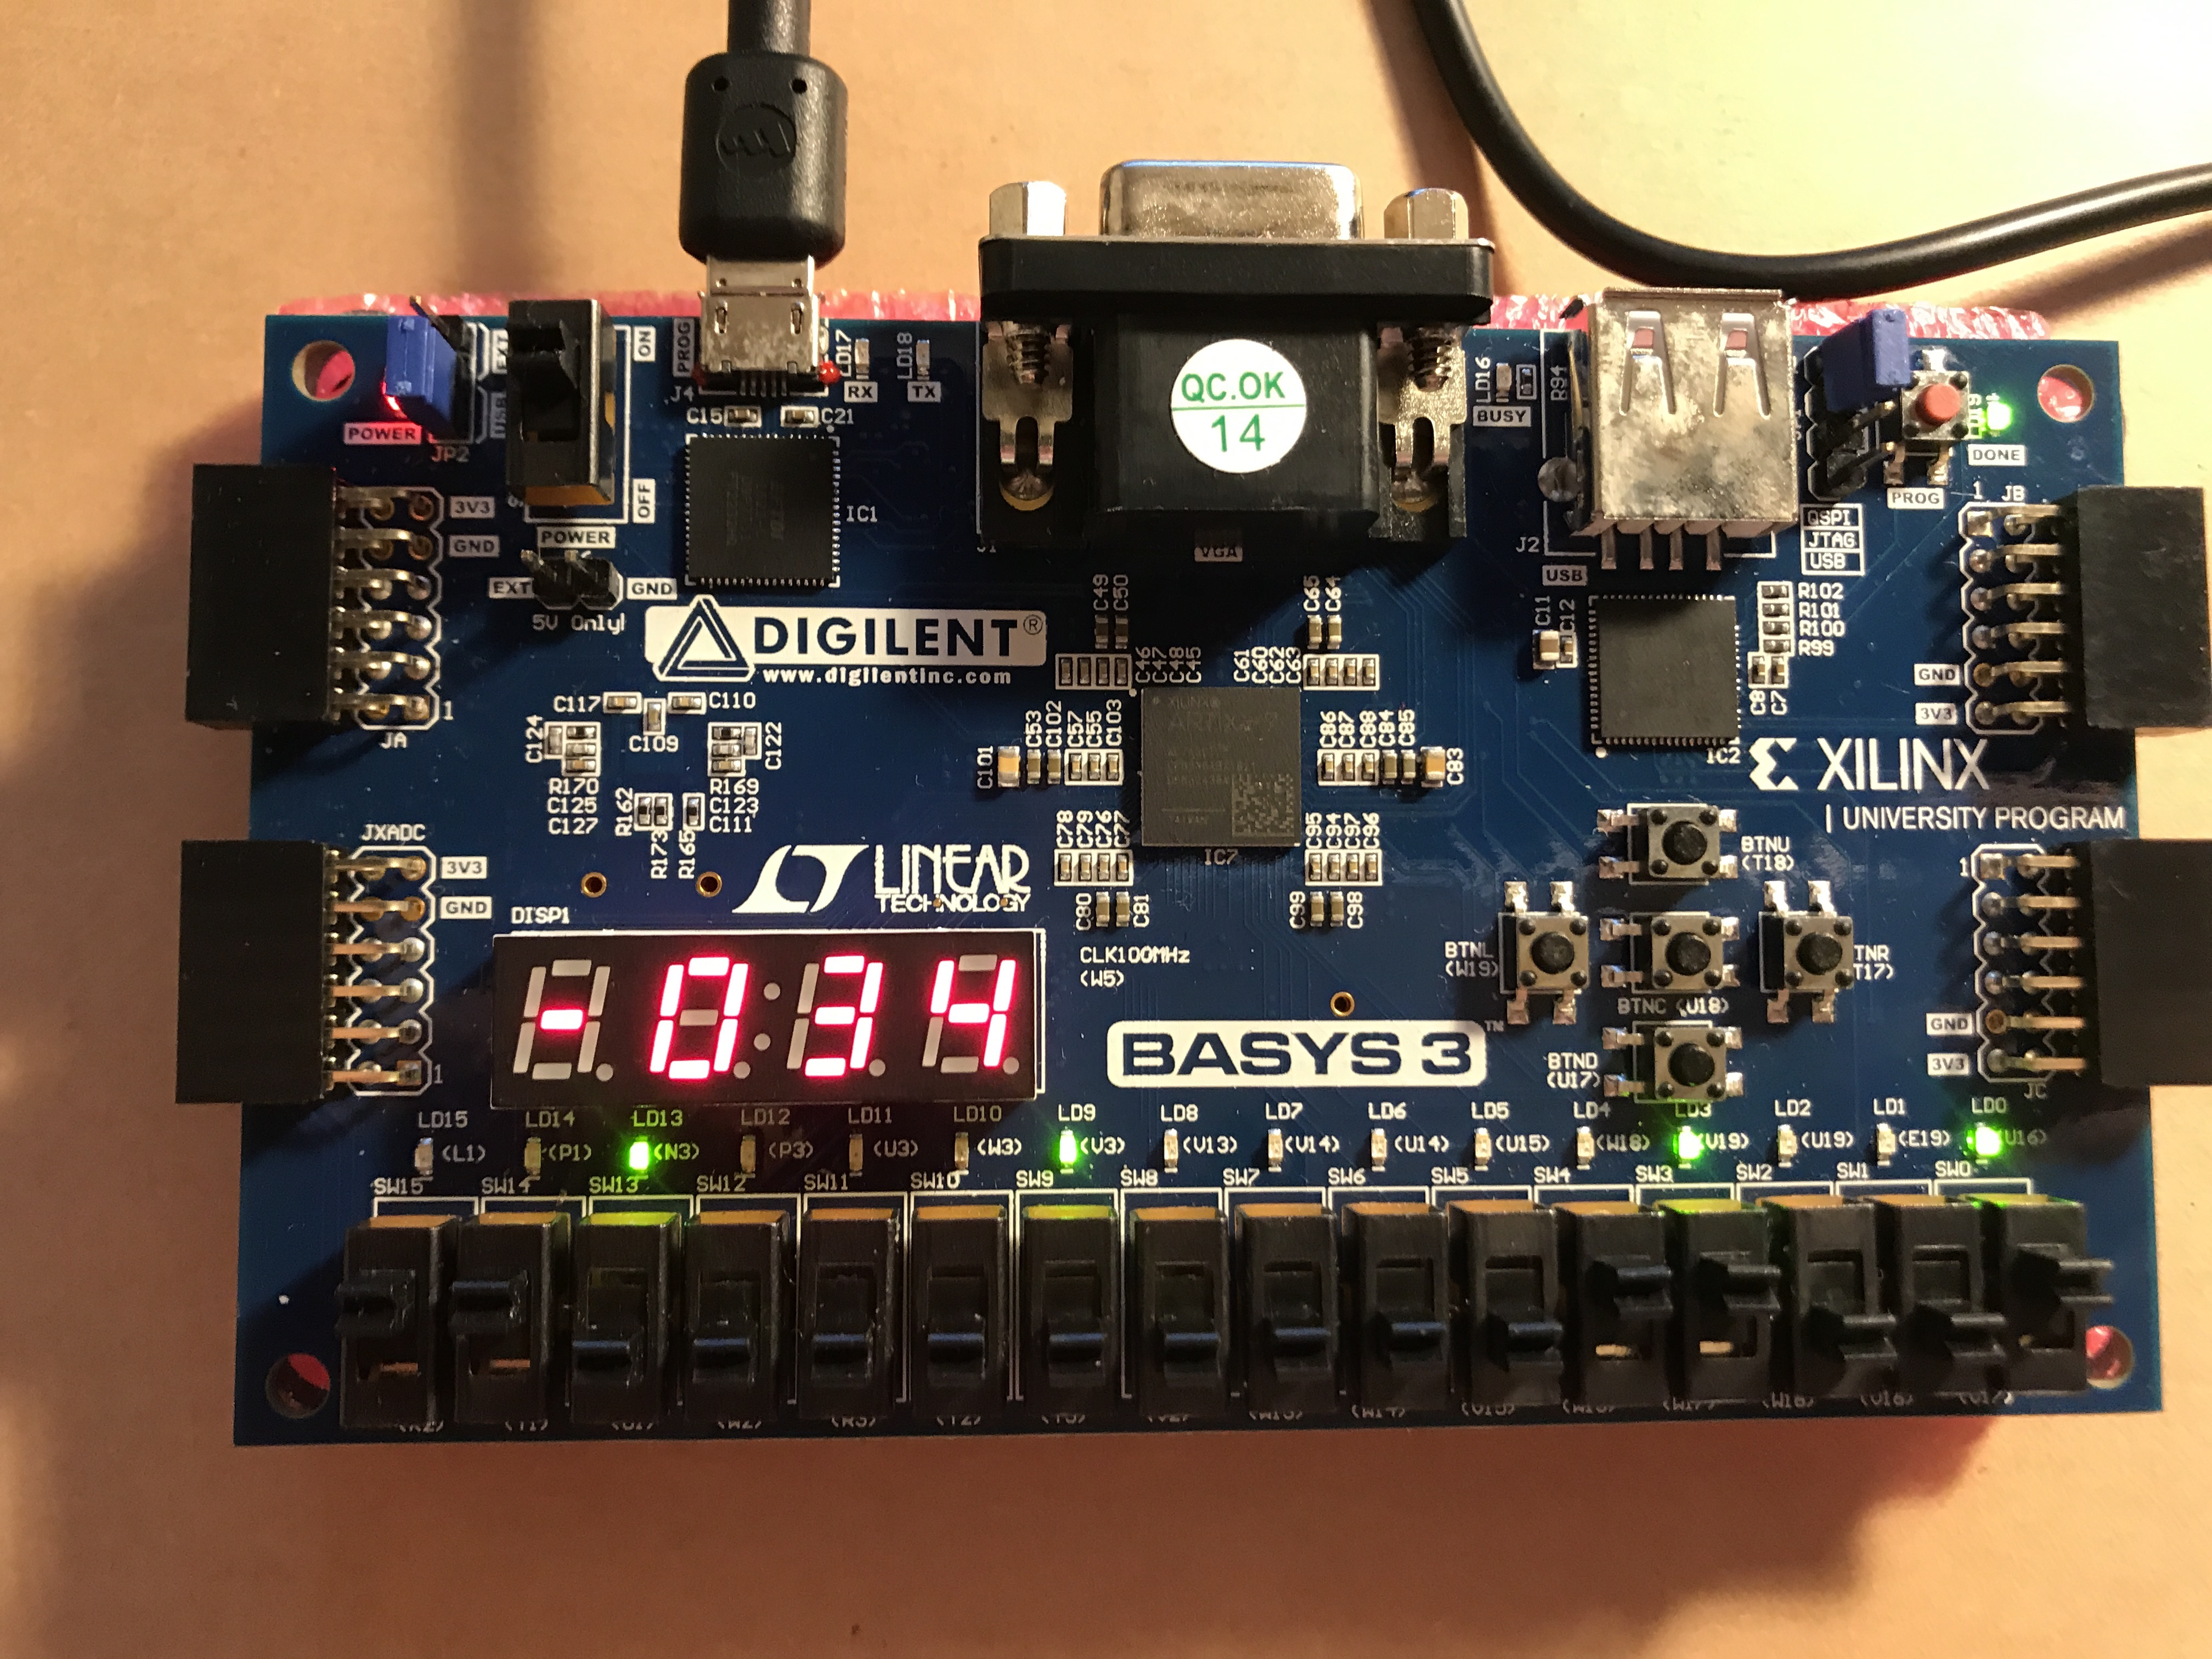
\includegraphics[width=0.5\textwidth]{board7}
	\caption{Board display 7.}
	\label{fig:board 7}			% label must be after caption
\end{figure}

\begin{figure}[ht]\centering
	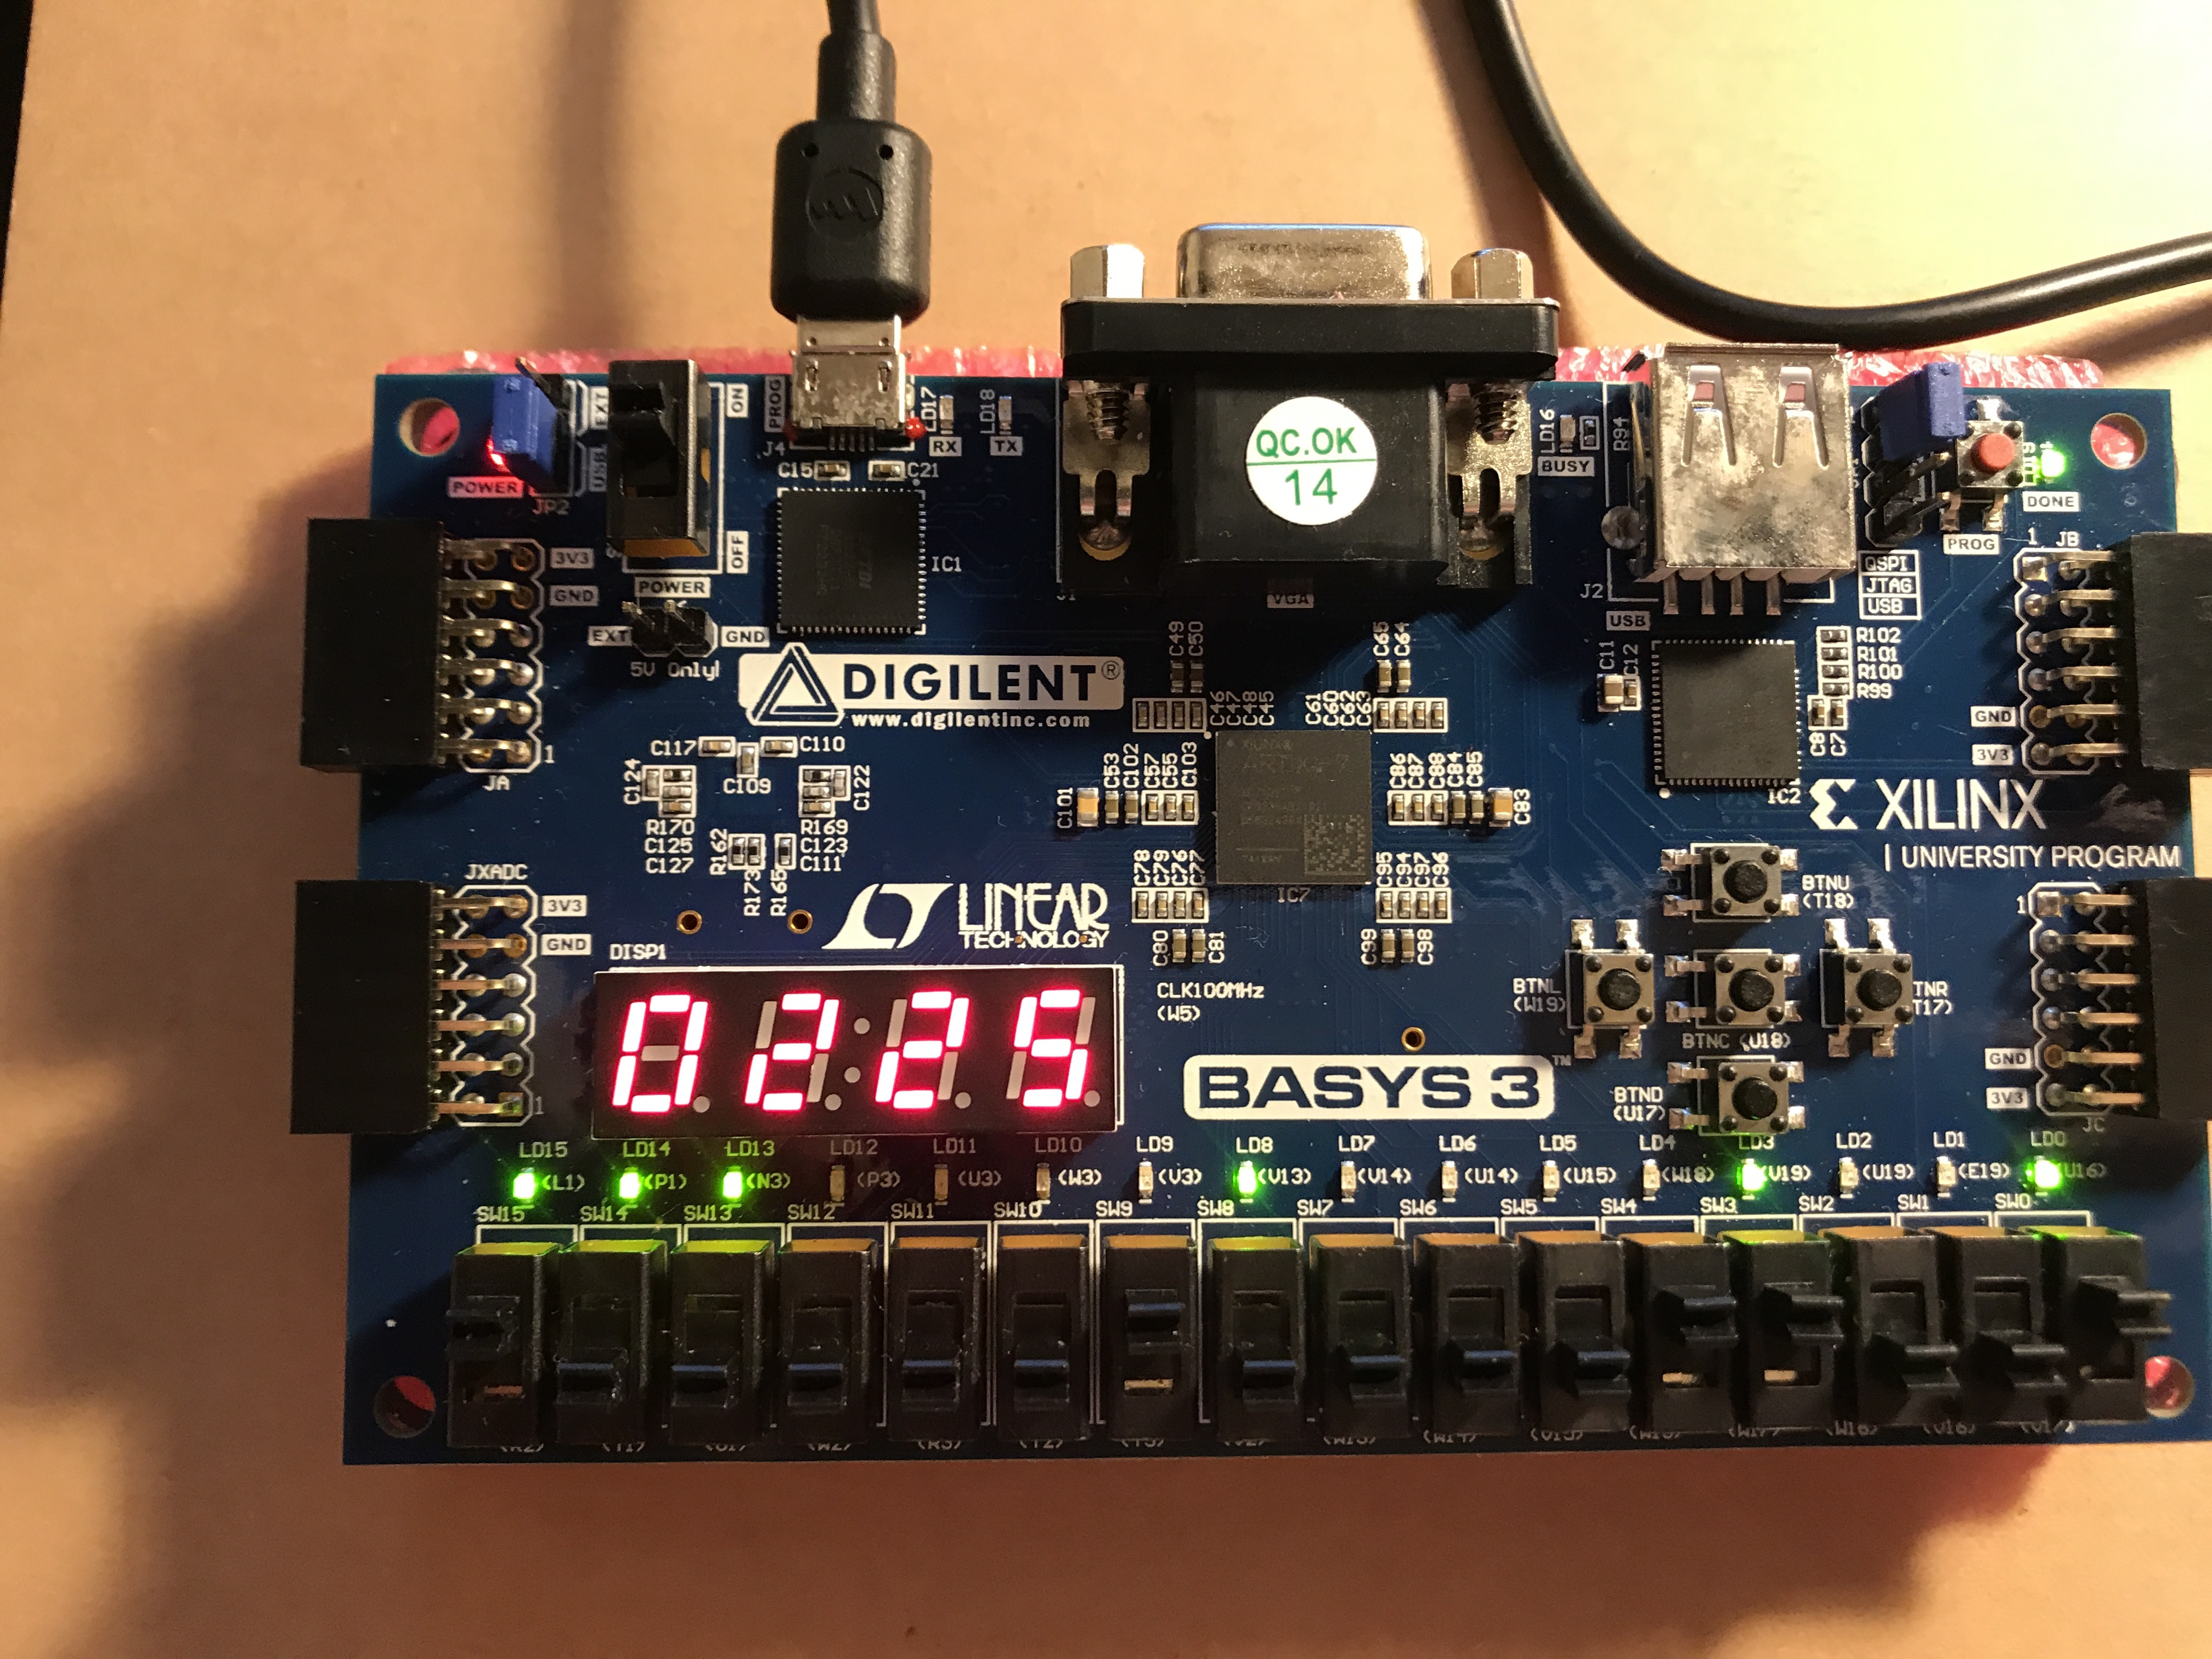
\includegraphics[width=0.5\textwidth]{board8}
	\caption{Board display 8.}
	\label{fig:board 8}			% label must be after caption
\end{figure}

\begin{figure}[ht]\centering
	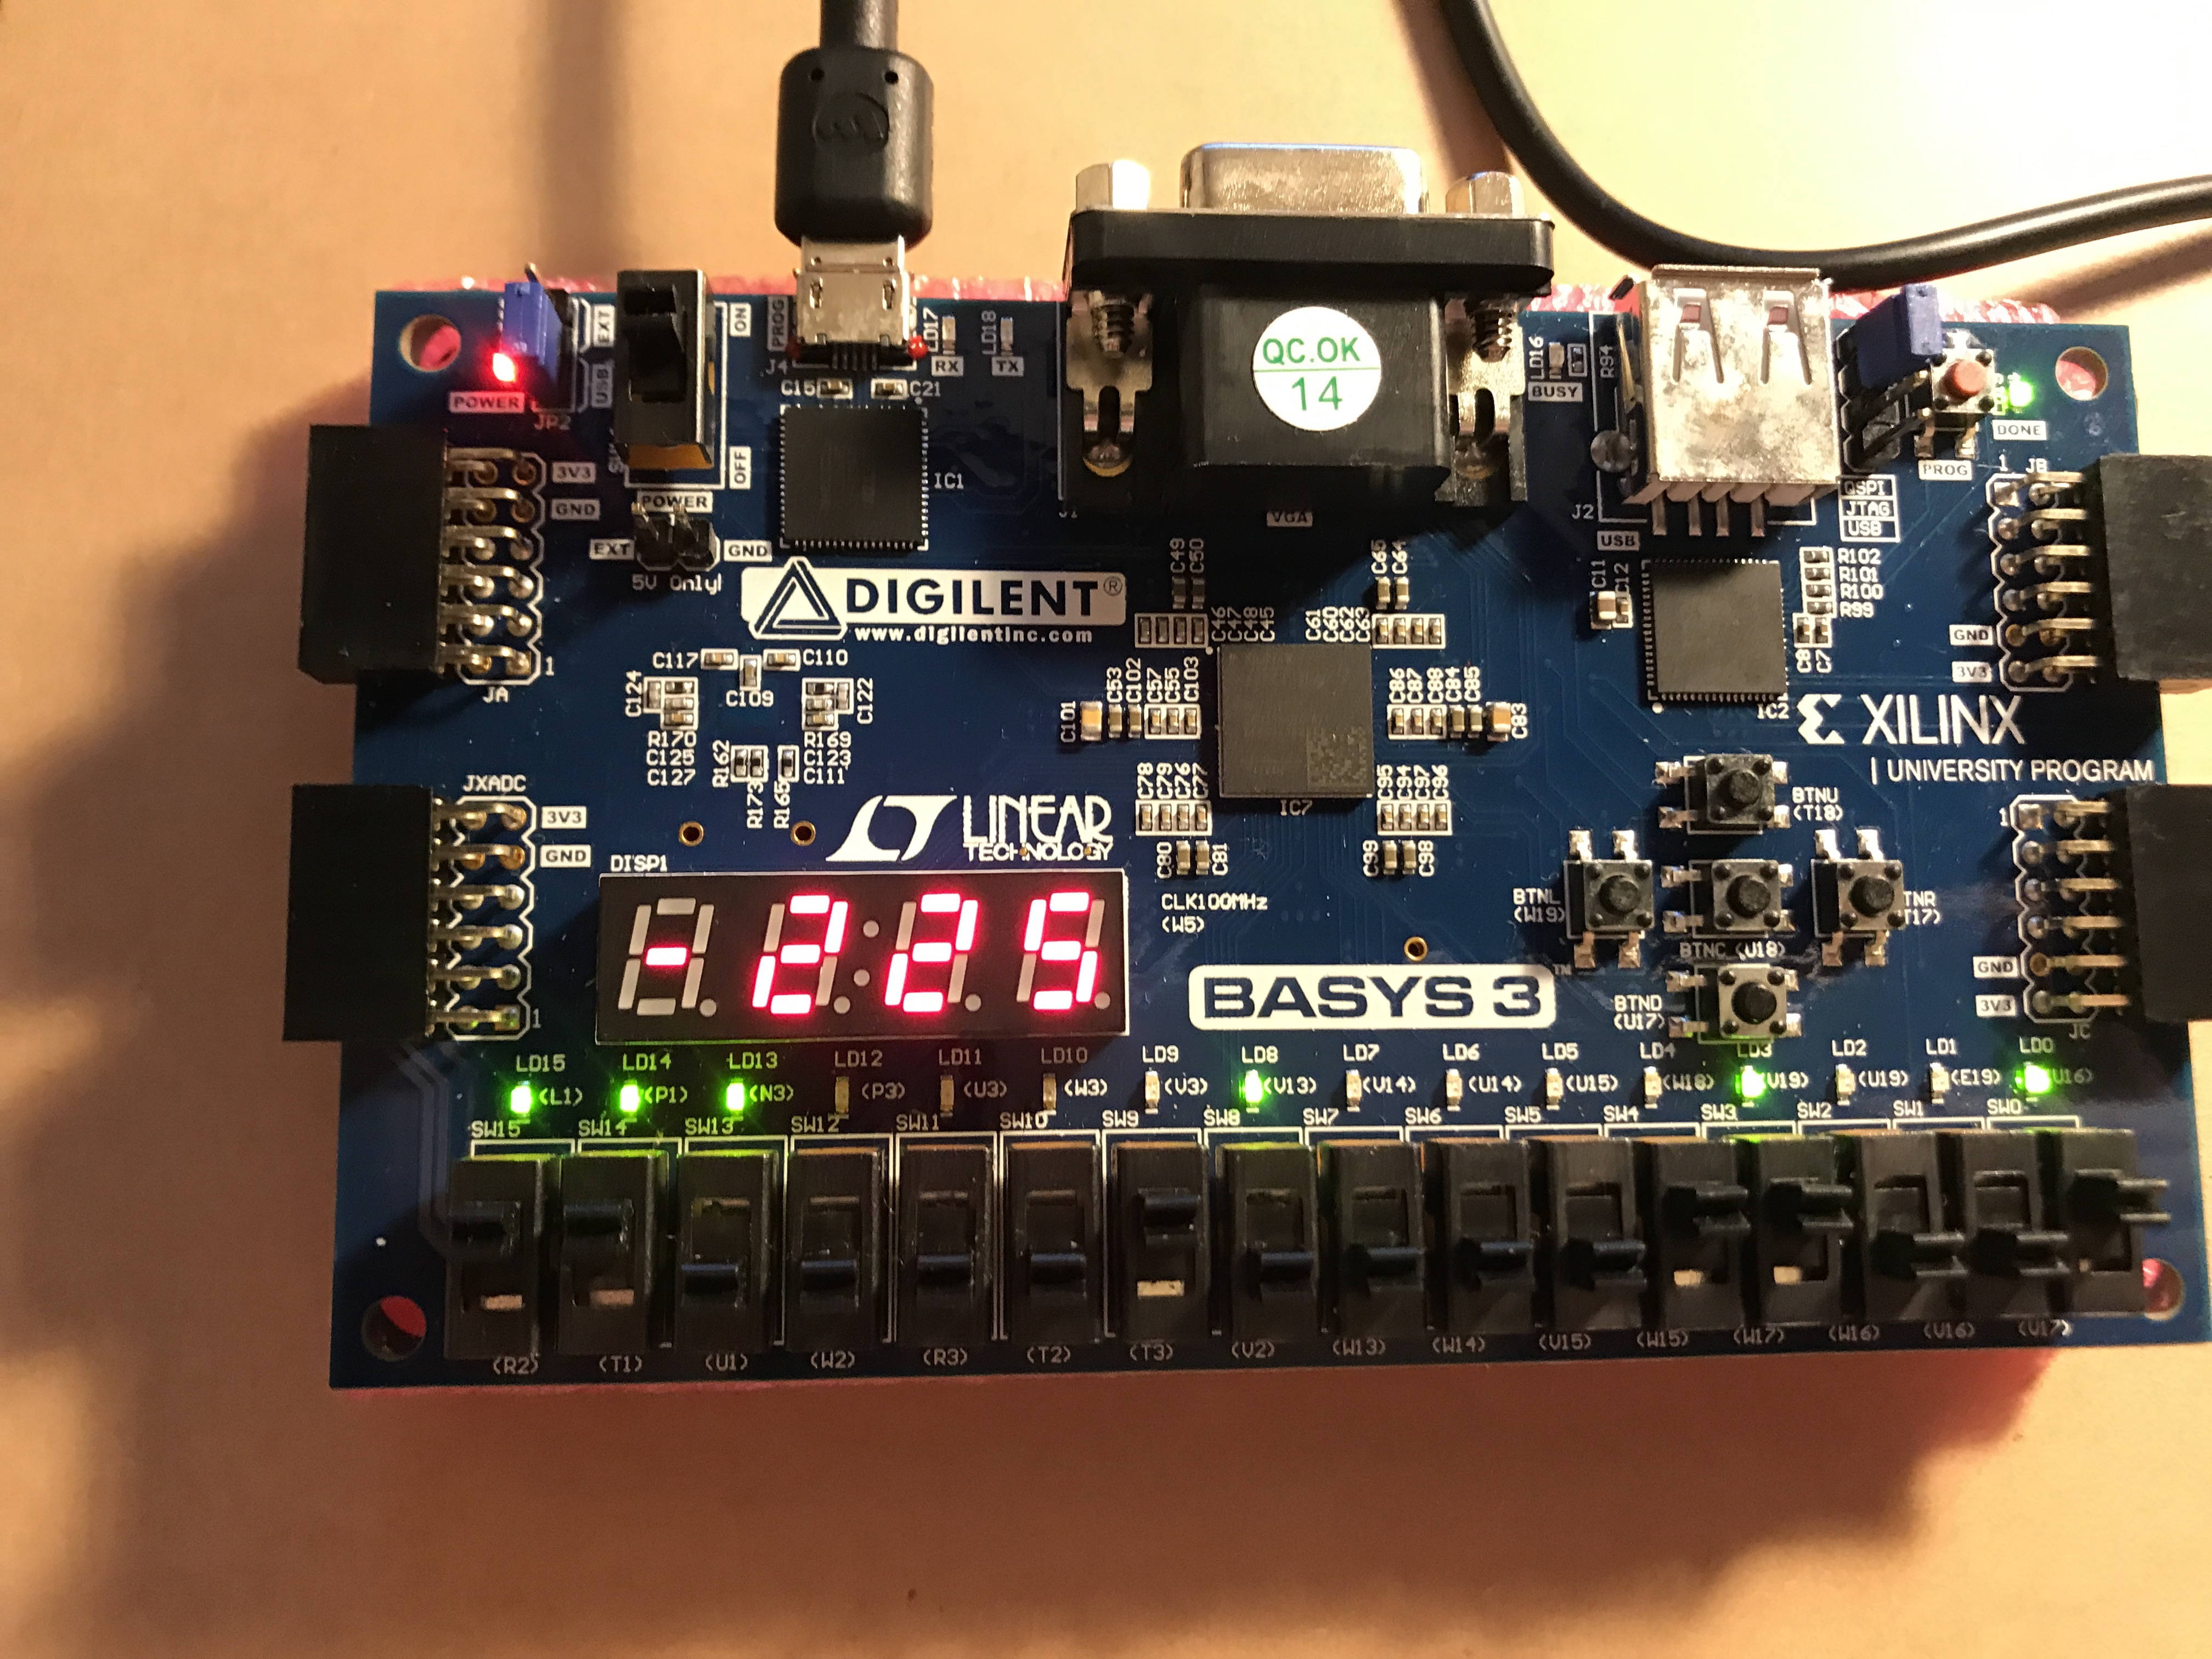
\includegraphics[width=0.5\textwidth]{board9}
	\caption{Board display 9.}
	\label{fig:board 9}			% label must be after caption
\end{figure}


\clearpage
\section*{Code}

\Verilog[firstline=23, lastline=53, caption=counter module source file,
label=code:counter]{counter.sv}

\Verilog[firstline=23, lastline=58, caption=sseg4 TDM module file,
label=code:mid-level]{sseg4_TDM.sv}

\Verilog[firstline=23, lastline=45, caption=calc lab10 module file,
label=code:top-level]{calc_lab10.sv}


\end{document}
